\documentclass{article}[12pt]
\usepackage{physics}
\usepackage{setspace}
\usepackage{amsmath}
\usepackage{mathrsfs}
\usepackage{amssymb}
\usepackage{feynmp-auto}
\usepackage{tgtermes}
\usepackage{graphicx}
\usepackage{booktabs}
\usepackage{array}
\usepackage{caption}
\usepackage{listings}
\usepackage{xcolor}
\usepackage{helvet}
\usepackage{float}
\definecolor{codegreen}{rgb}{0,0.6,0}
\definecolor{codegray}{rgb}{0.5,0.5,0.5}
\definecolor{codepurple}{rgb}{0.58,0,0.82}
\definecolor{backcolour}{rgb}{0.95,0.95,0.92}
\definecolor{lightgray}{rgb}{0.95,0.95,0.95}

\lstdefinestyle{mystyle}{
    backgroundcolor=\color{lightgray},   
    commentstyle=\color{codegreen},
    keywordstyle=\color{magenta},
    numberstyle=\tiny\color{codegray},
    stringstyle=\color{codepurple},
    basicstyle=\fontfamily{pcr}\selectfont\footnotesize,
    breakatwhitespace=false,         
    breaklines=true,                 
    captionpos=b,                    
    keepspaces=true,                 
    numbers=left,                    
    numbersep=5pt,                  
    showspaces=false,                
    showstringspaces=false,
    showtabs=false,                  
    tabsize=2
}
\setcounter{page}{29}
\setcounter{figure}{13}
\setcounter{table}{2}
\setcounter{section}{3}
\lstset{style=mystyle}
\captionsetup{font=footnotesize}
\newcommand{\RN}[1]{%s
  \textup{\uppercase\expandafter{\romannumeral#1}}%
}
\usepackage{geometry}
\geometry{
 a4paper,
 left=25.4mm,
 right=25.4mm,
 top=30mm,
 bottom=25.4mm
 }
\begin{document}
\section{Result}
\begin{spacing}{1.5}
\subsection{Summary}
  To investigate the physical changes occurring in the Josephson junction based on the results of the previous sections,  
  we used two methods to analyze the calculation result. The first involved examining the changes in the order parameter, $\cos{\phi}$. 
  As a second method, we calculate the correlation function between the excited and ground states, and express it using an approximation formula for phase based on fluctuation-dissipation theory. 
  To evaluate the accuracy of the calculated results, 
  we tested each section of the integration code by comparing it with the case without reservoir effects, 
  comparing it with higher-order approximation methods, and checking for convergence depending on the calculation conditions.
\subsection{Benchmark}
\subsubsection*{Exact diagonalization in single mode}
To compare with the result from exact diagonalization(ED), we set the condition when the bath has only a single mode. 
The result shows approximation method could be reliable in high temperatures ($\beta = 1$).
\begin{figure}[htbp]
  \centerline{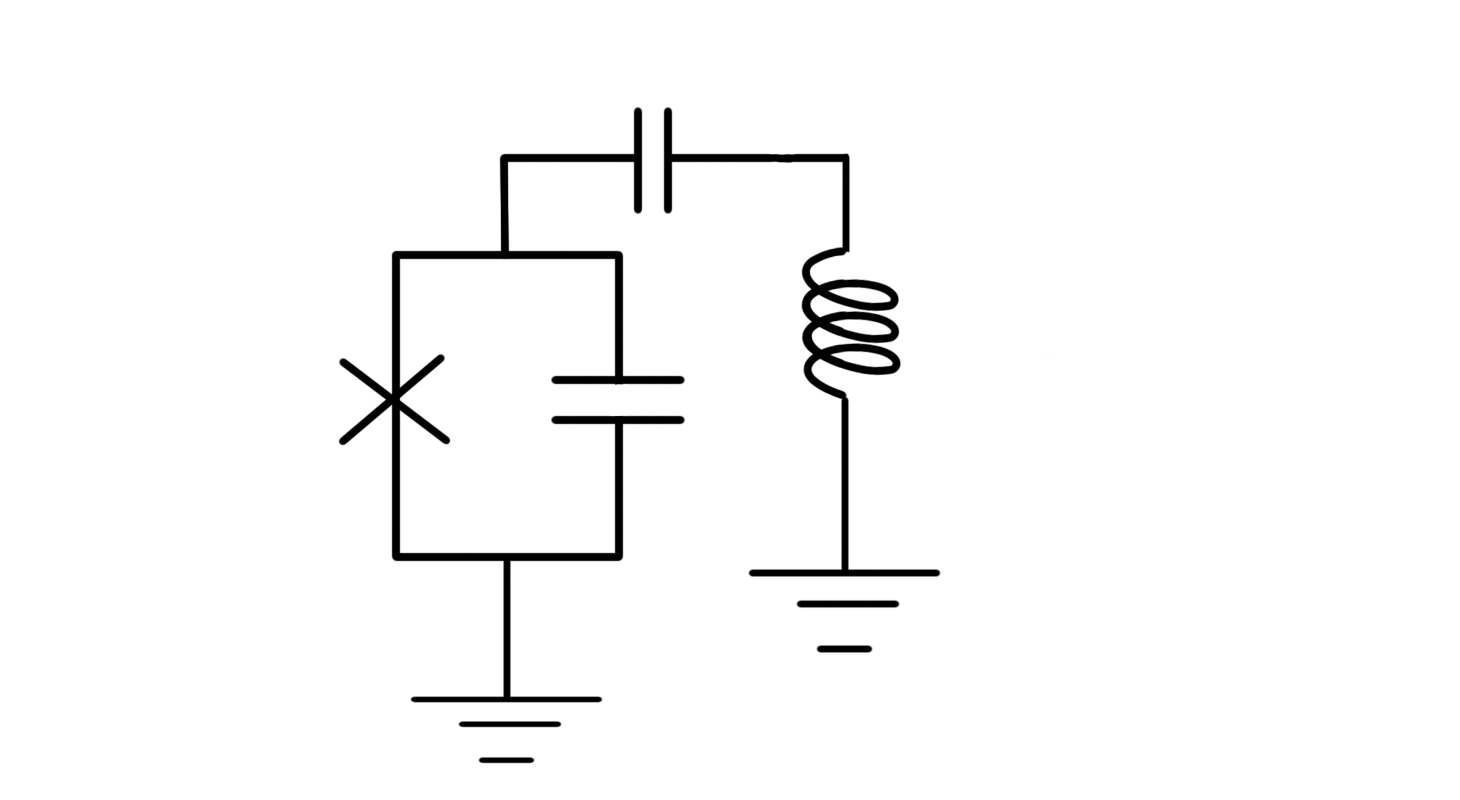
\includegraphics[width=7cm]{TexFigure/kps_singlebath.png}}
  \caption{Brief circuit scheme for single bath condition. The crossing symbol  refers to the insulated junction of Josephson junction.}
\end{figure}
\begin{figure}[htbp]
  \centerline{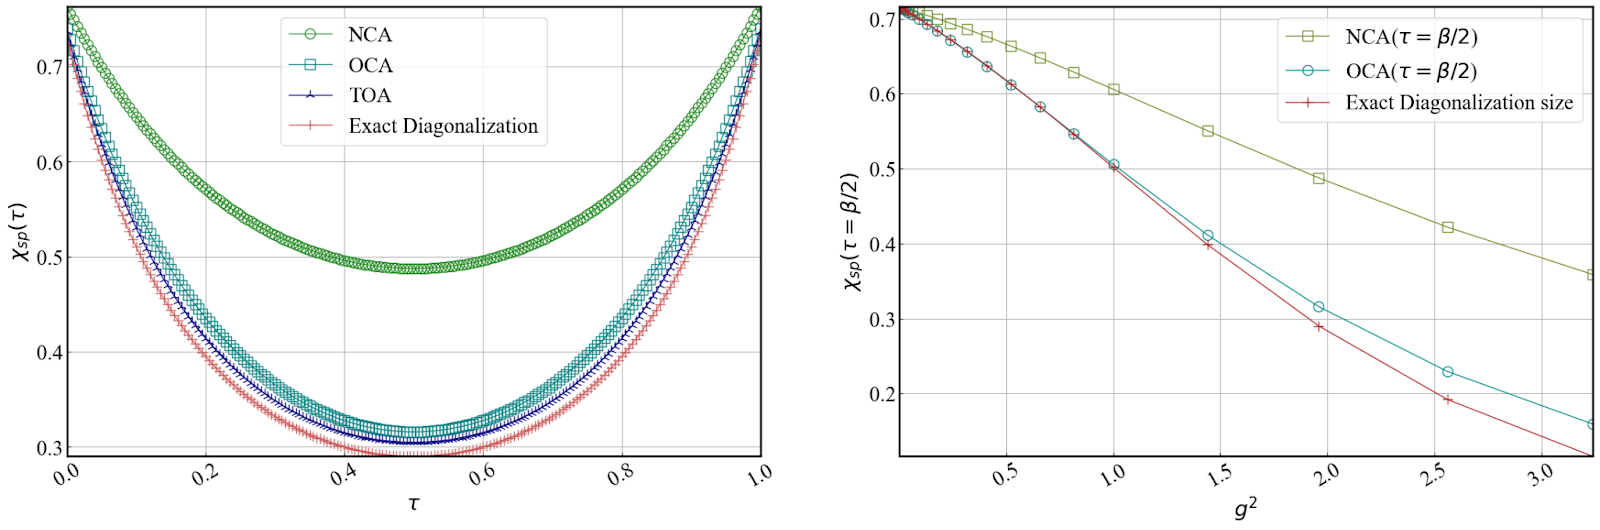
\includegraphics[width=15cm]{TexFigure/bench_single_two.png}}
  \caption{Result for single bath benchmark. For $\chi_{sp} - \tau$(Left), it conducted on overall condition g (coupling strength with system-bath) = 1.
  With $\chi_{sp}(\tau=\beta/2)-g^2$(Right), It shows that if order of perturbation increases, the results approach the exact results.}
\end{figure}
\subsubsection*{Multi-mode case}
To investigate the convergence of the diagrammatic approximation method in a general bosonic reservoir condition, 
we calculated the order parameter and the correlation function using the NCA, OCA, and TOA. 
The results showed no significant difference between the OCA and TOA calculations, confirming that the OCA is a sufficiently convergent method.
\begin{figure}[H]
  \centerline{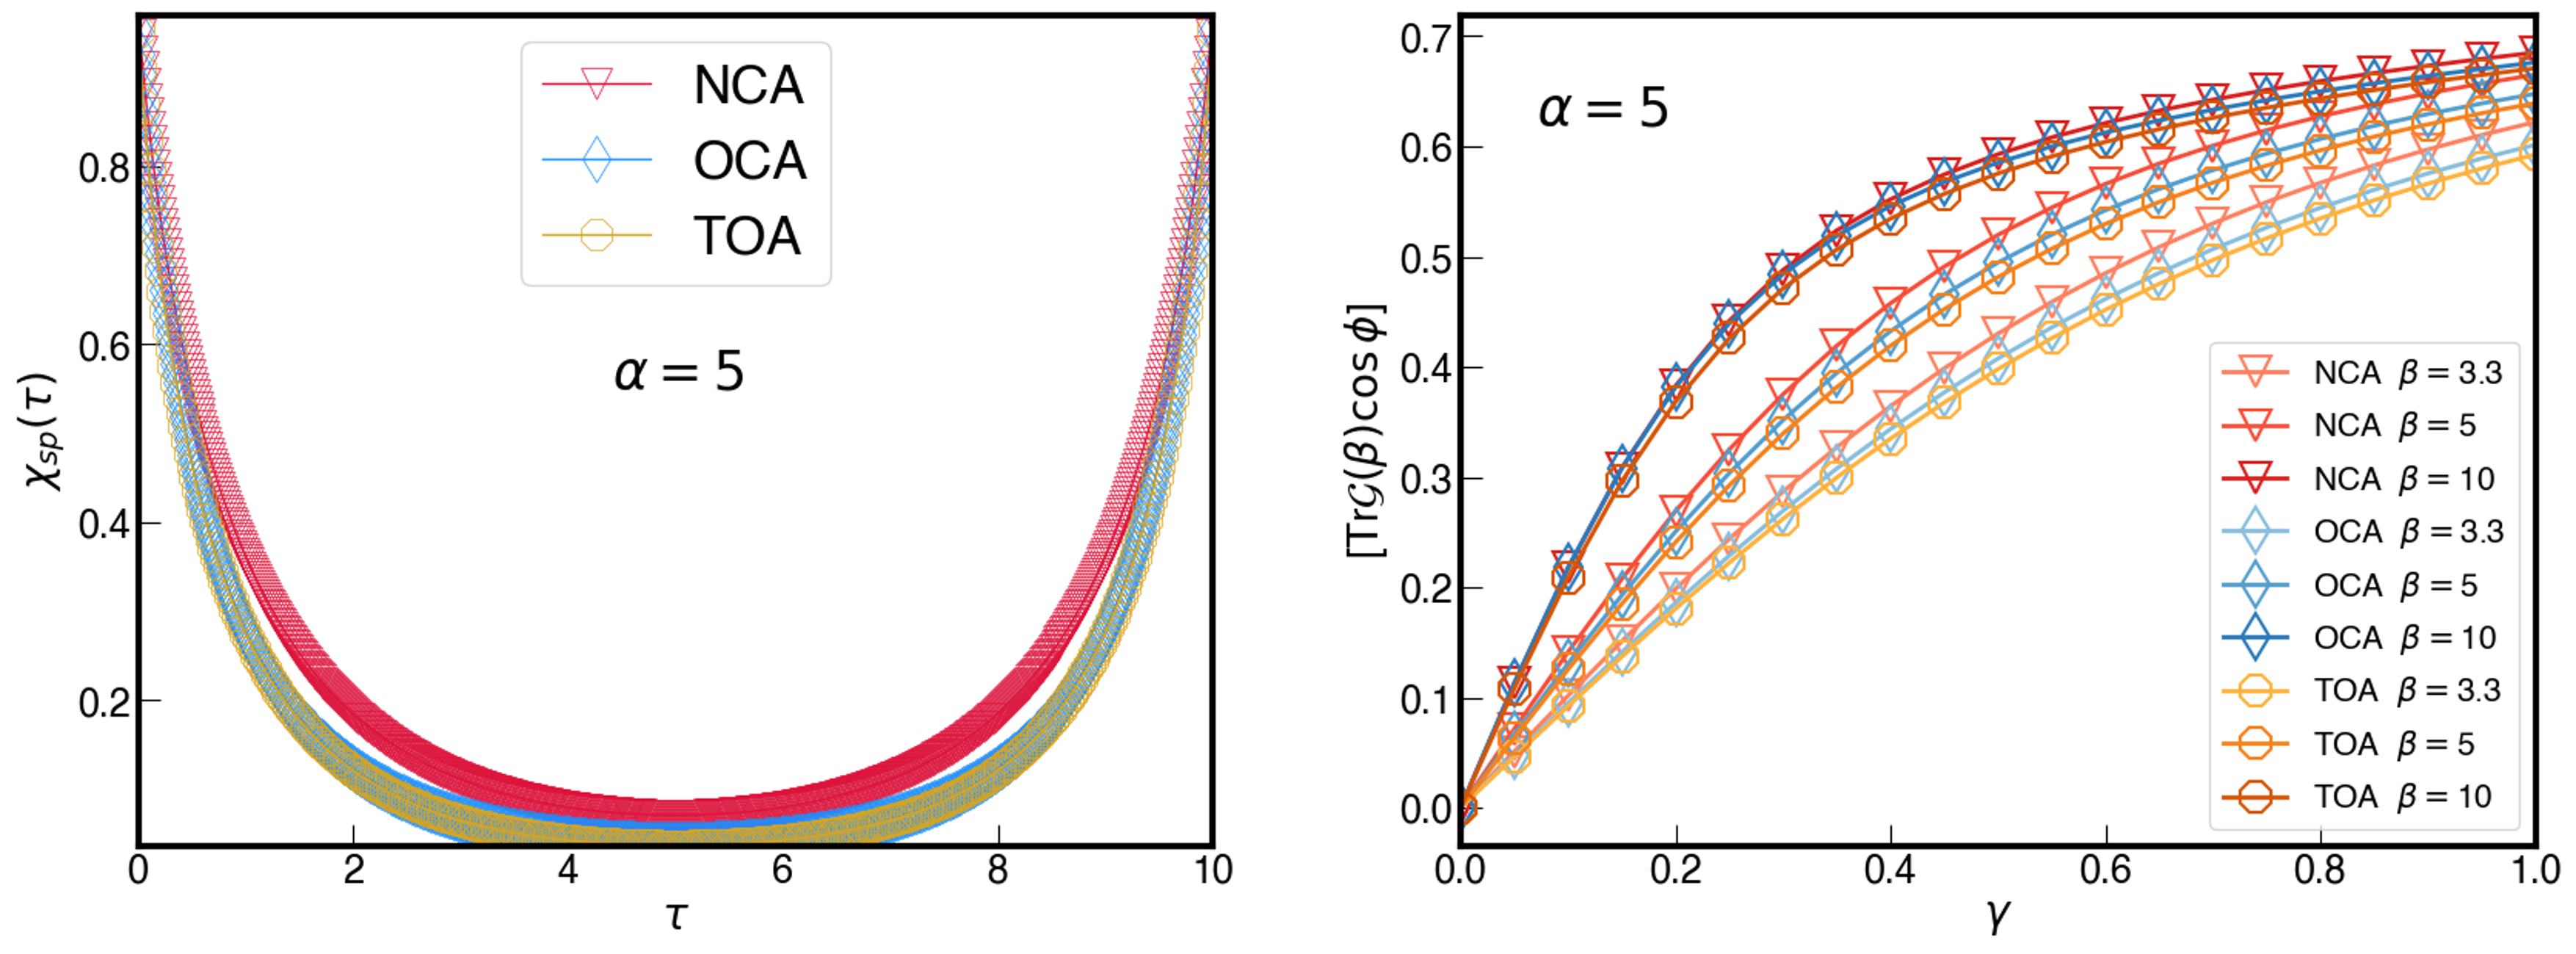
\includegraphics[width=15cm]{TexFigure/Multi_bench.png}}
  \caption{ Calculation results of the order parameter and correlation function using each order of the approximation method. 
  Both figures are for the case of $\alpha$=5, with the left figure showing temperatures between 0.3 and 0.1, 
  the right figure is for the temperature condition of 0.1. It can be observed that the calculation results of OCA and TOA are converged. 
  The size of the τ grid used for the calculation is 701.}
\end{figure}
\subsubsection*{Benchmarking solver code in $\alpha$ = 0 condition}
To check for the integration code, we compared the order parameter calculated using approximation methods for the case of α=0 
with the order parameter calculated using the state density matrix of the Josephson junction system. 
The results showed that the two cases were completely consistent.
\begin{figure}[H]
  \centerline{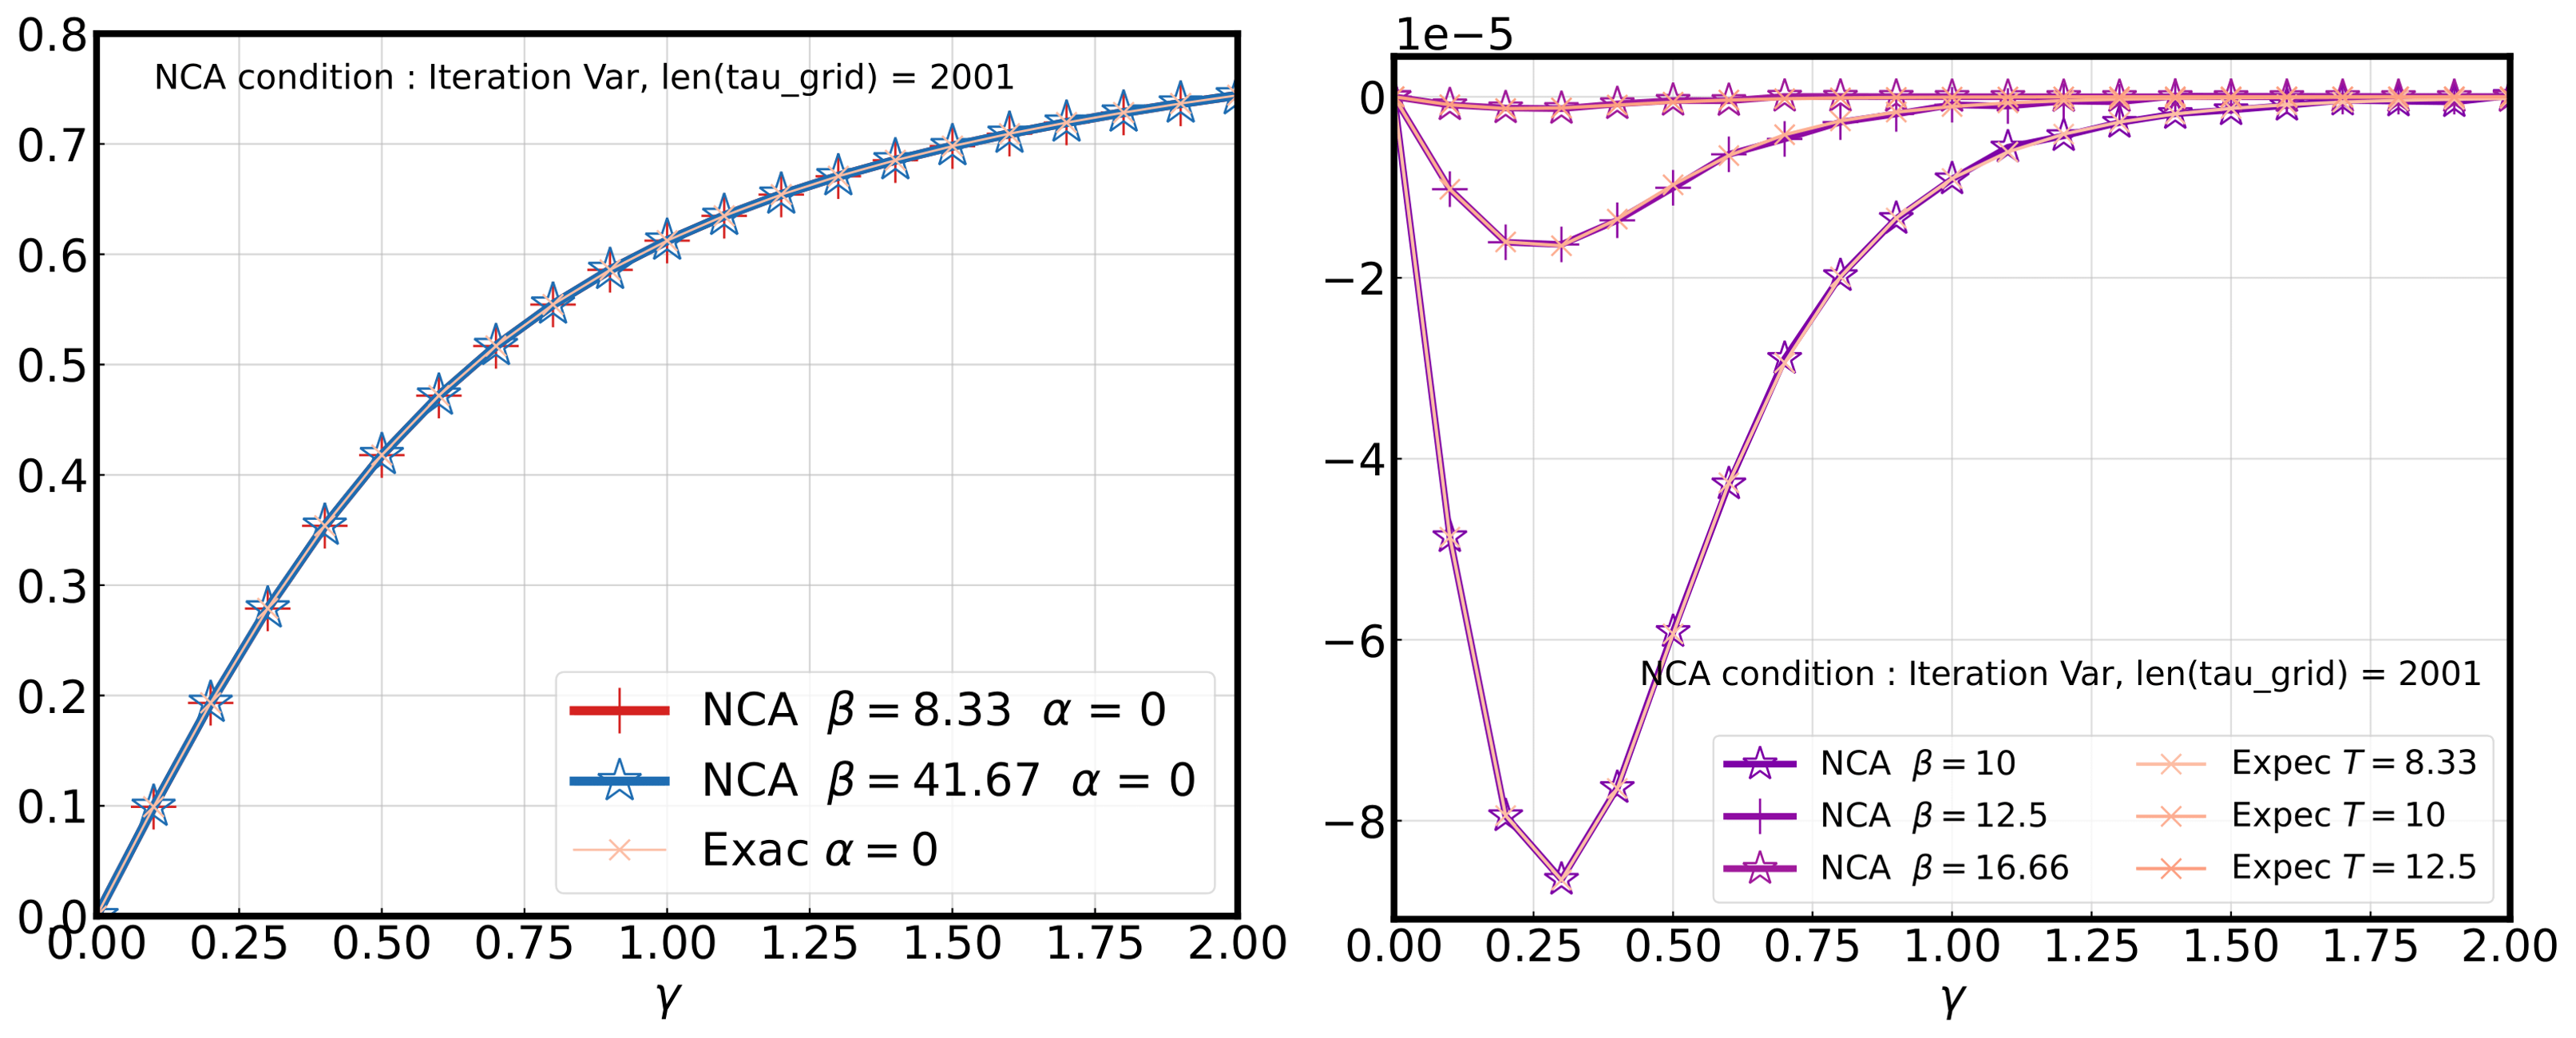
\includegraphics[width=15cm]{TexFigure/Dens_comp.png}}
  \caption{In the case of $\alpha = 0$, order parameter calculation using the approximation method should be consistent with using $H_{loc}$.
  The comparison confirmed that the two cases show consistency. The left figure shows the calculation of the order parameter, 
  and the right figure shows the difference in the order parameter for consecutive $\beta$ values,
   in the intervals [8.33, 10], [10, 12.5], and [12.5, 16.6].}
\end{figure}
\pagebreak
\subsection{Simulation condition}
The control parameters are as follows: $\gamma$ represents the nonlinearity of the Josephson junction system, 
$\alpha$ represents the interaction with the external environment. Regarding the previous study which has been reported 
that the transition occurs at $\alpha = 1$, we set the range of parameters around $\alpha = 1$ and $\gamma = 1$ . 
The factors influencing the accuracy of the approximation method are the number of integration iterations and the size of the $\tau$ grid. 
We set the range of variables used in the simulation as Table 2 and Table 3.
\begin{table}[htbp]
  \centering
  \renewcommand{\arraystretch}{1.2}  % 행 간격 조정
  \begin{tabular}{@{}cccc@{}}
  \toprule
  \textbf{Variables} & \textbf{Min} & \textbf{Max}  & \textbf{Interval}\\ 
  \midrule
  $\gamma$ & 0 & 2 & 0.1 \\
  $\alpha$ & 0 & 2 & 0.01 \\
  $\beta$ & 7.14 & 62.5 &  \\
  Temperature & 0.016 & 0.14 & 0.02 (until 0.04) \\
  \bottomrule
  \end{tabular}
  \caption{Parameter interval used for calculation.}
  \end{table}
\begin{table}[htbp]
  \centering
  \renewcommand{\arraystretch}{1.2}  % 행 간격 조정
  \begin{tabular}{@{}ccc@{}}
  \toprule
  \textbf{Number} & \textbf{Interval} & \textbf{Gridsize}\\ 
  \midrule
  $\tau$ grid & [0,$\beta$] & 2000 \\
  k grid & [0,K = 30000] & 30000 \\
  \bottomrule
  \end{tabular}
  \caption{Grid condition used for calculation.}
  \end{table}
\subsubsection*{Saturation test}
We investigated the convergence behavior of the calculation results for the change of the order parameter. 
We were able to confirm that the results converge for the case of a tau grid size of 1800 to 2000. 
\begin{figure}[htbp]
  \centerline{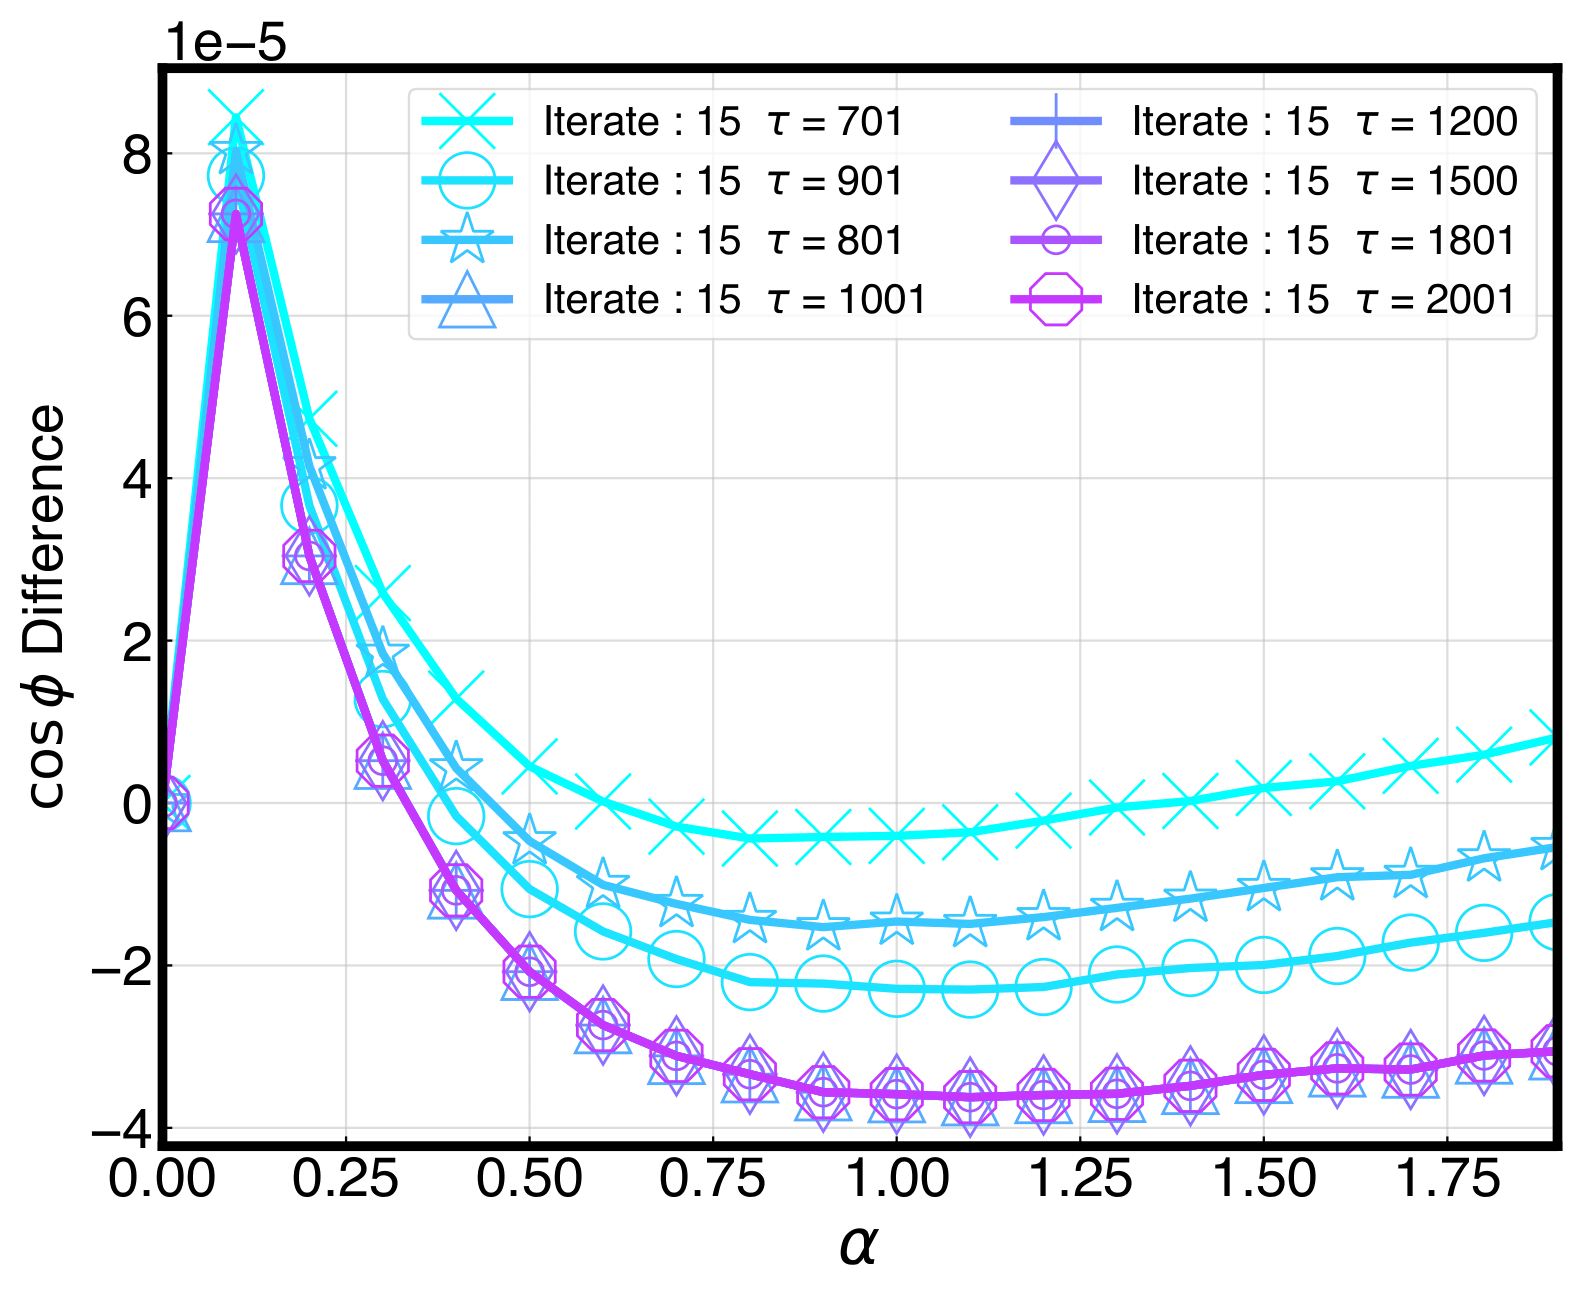
\includegraphics[width=10cm]{TexFigure/Diff_Ns3_g_b_35.71_41.67_n_15_tauchange (1)-1.png}}
  \caption{Saturation test in different time grid size. The temperature condition is $\beta = 41.67$}
\end{figure}
\subsubsection*{Size dependence}
Since the resistively shunted Josephson junction circuit corresponds to a model that the physical system has coupled to waveguide structure,
there was a breakdown of the rotating wave approximation of the two-level system as the coupling strength between the RC resonator circuit 
and the Josephson junction increases[15]. The test condition is $\gamma =2$ , $\alpha = 1.5$ with calculating correlation function. 
From the benchmark result, adopting 2-level truncated condition is reliable since the difference between two size is ignorable.
\begin{figure}[H]
  \centerline{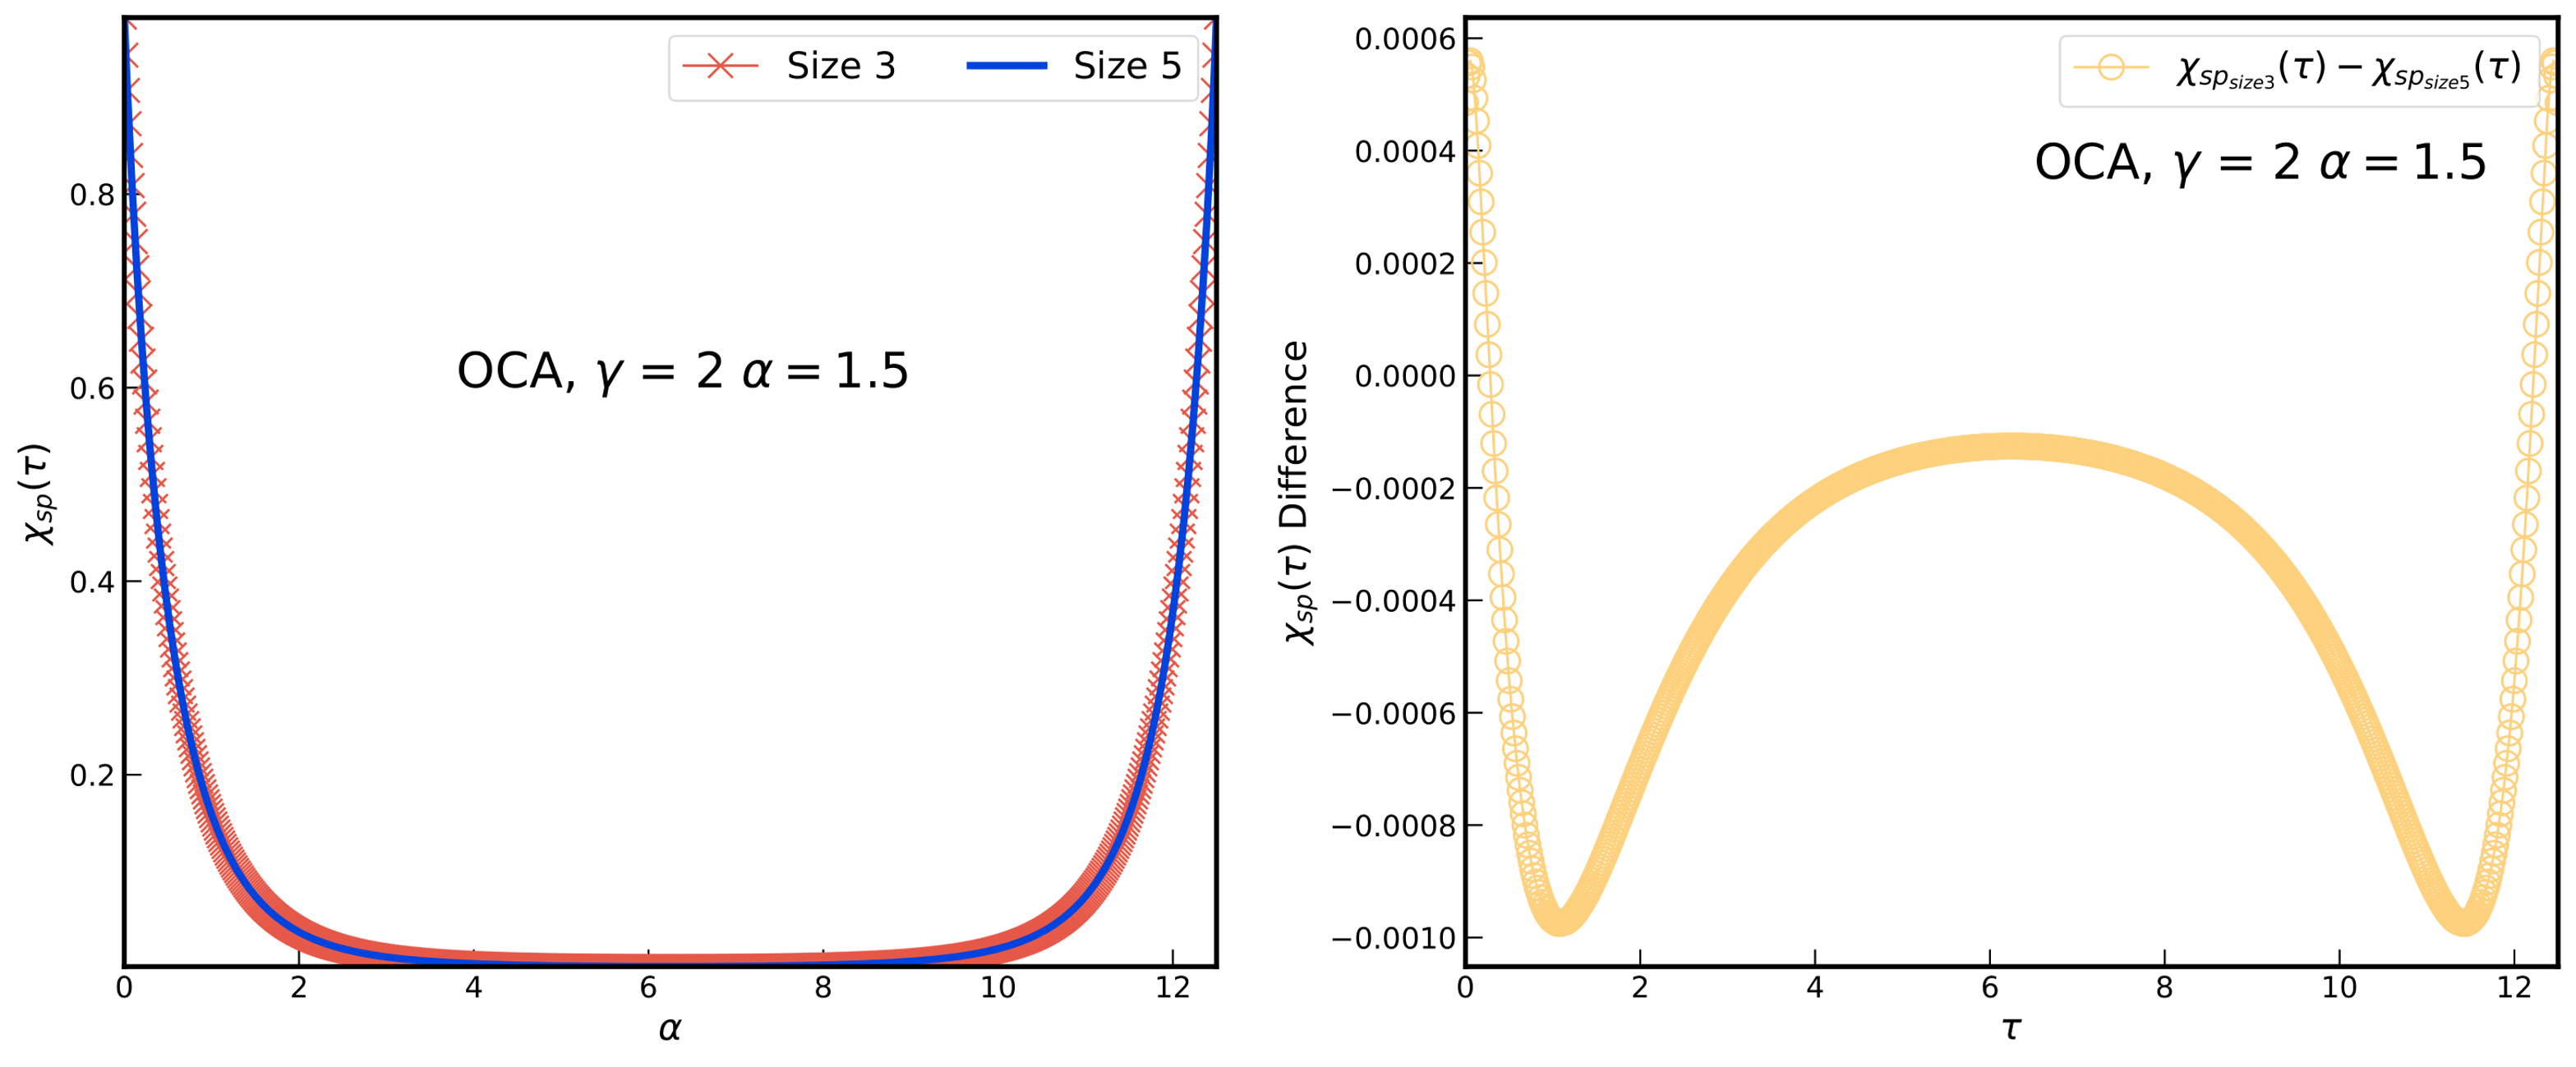
\includegraphics[width=15cm]{TexFigure/Sizediff.png}}
  \caption{Comparision with $\chi_{sp}(\tau)$ size3 and size5. The size of $\tau$ grid is 700.}
\end{figure}
\pagebreak
\subsection{Orderparmeter evaluation}
\subsubsection*{Orderparameter}
First, we calculated the expectation value of the order parameter $\hat{\cos\phi}$, 
over the given range of $\gamma$. The results showed that the Josephson junction exhibited superconducting behavior 
as its nonlinearity increased at all temperatures. Subsequently, we compared the diagonal elements of the product 
of the operator $\hat{\cos\phi}$ and the operator $\hat{H_{\text{loc}}}$ , both expressed in matrix form, 
for different degrees of coupling with the external environment. We expected that the probability of the system 
being in the ground state would be the highest for all three $\alpha$ values. From the result, 
it can be deduced that the system is localized that corresponds with the superconductor state which is consistent with observed
result from the expectation value of the order parameter.
\begin{figure}[htbp]
  \centerline{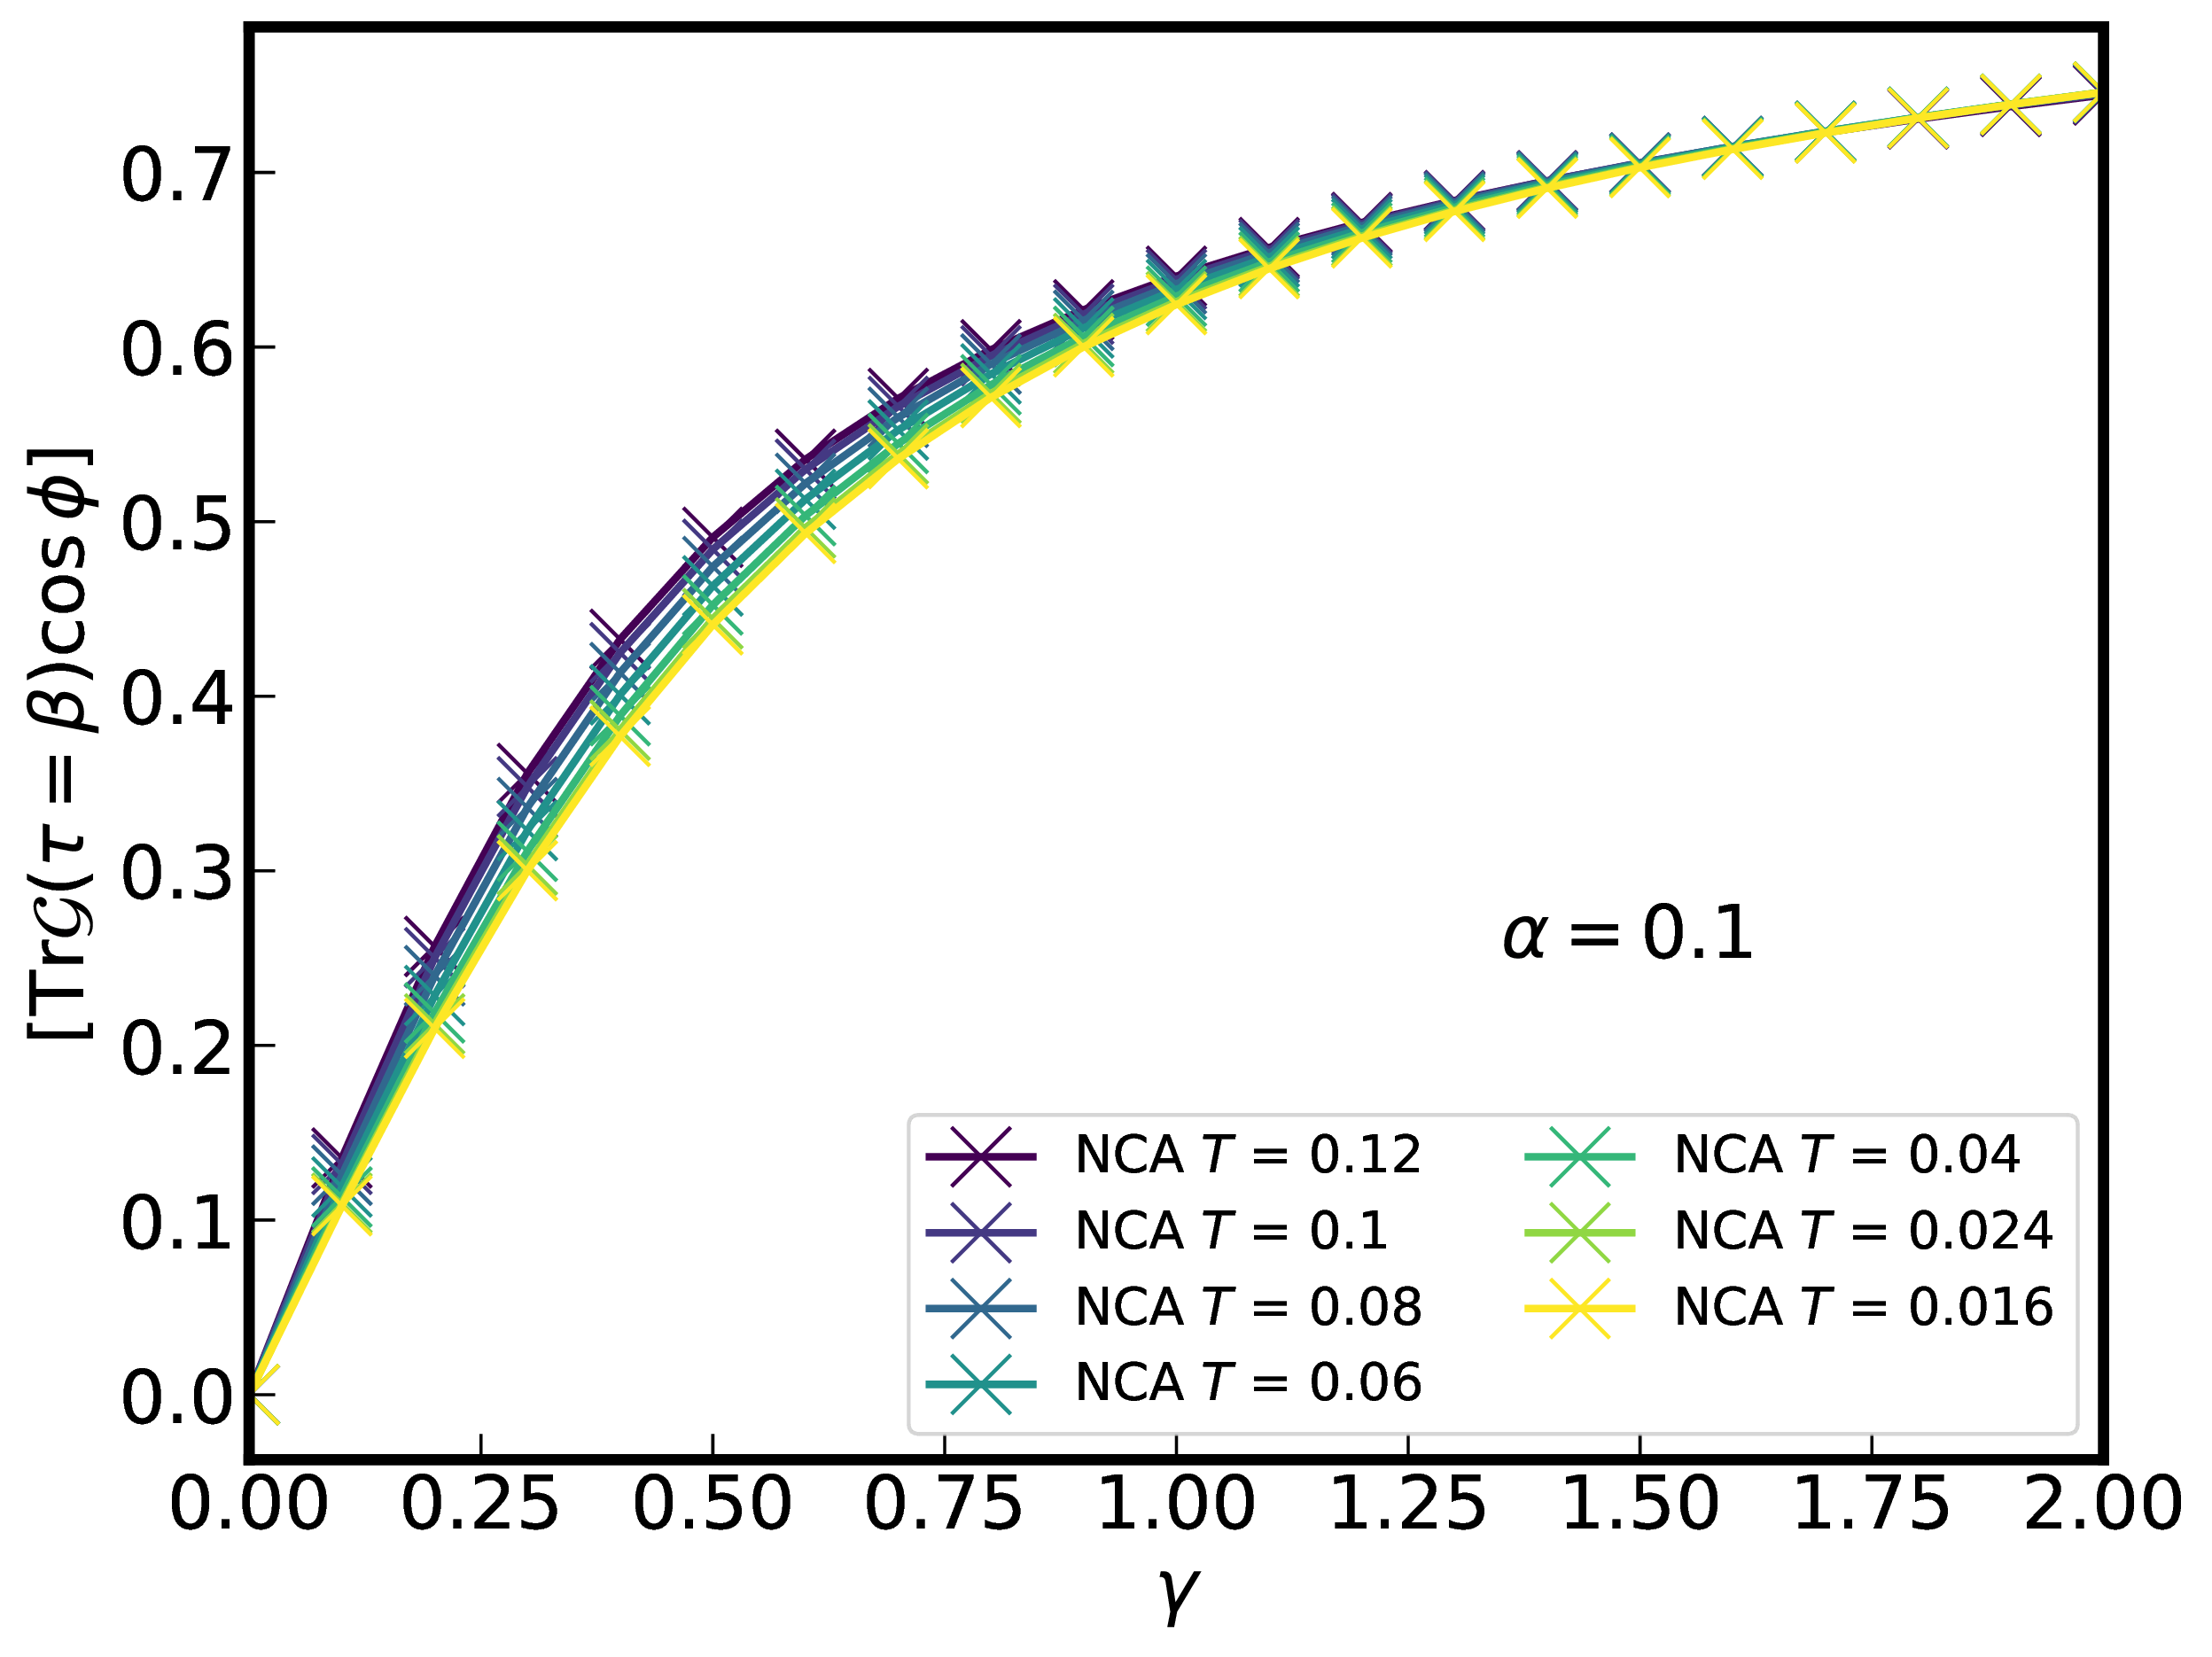
\includegraphics[width=10cm]{TexFigure/Expec_alp_0.1.png}}
  \caption{Calculation of the expectation value of the order parameter for the case of $\alpha$=0.1. 
  The expectation value of the order parameter varies with temperature in the range of $\gamma$ ≈[0,1.5].}
  \label{fig:Order1}
\end{figure}
\begin{figure}[htbp]
  \centerline{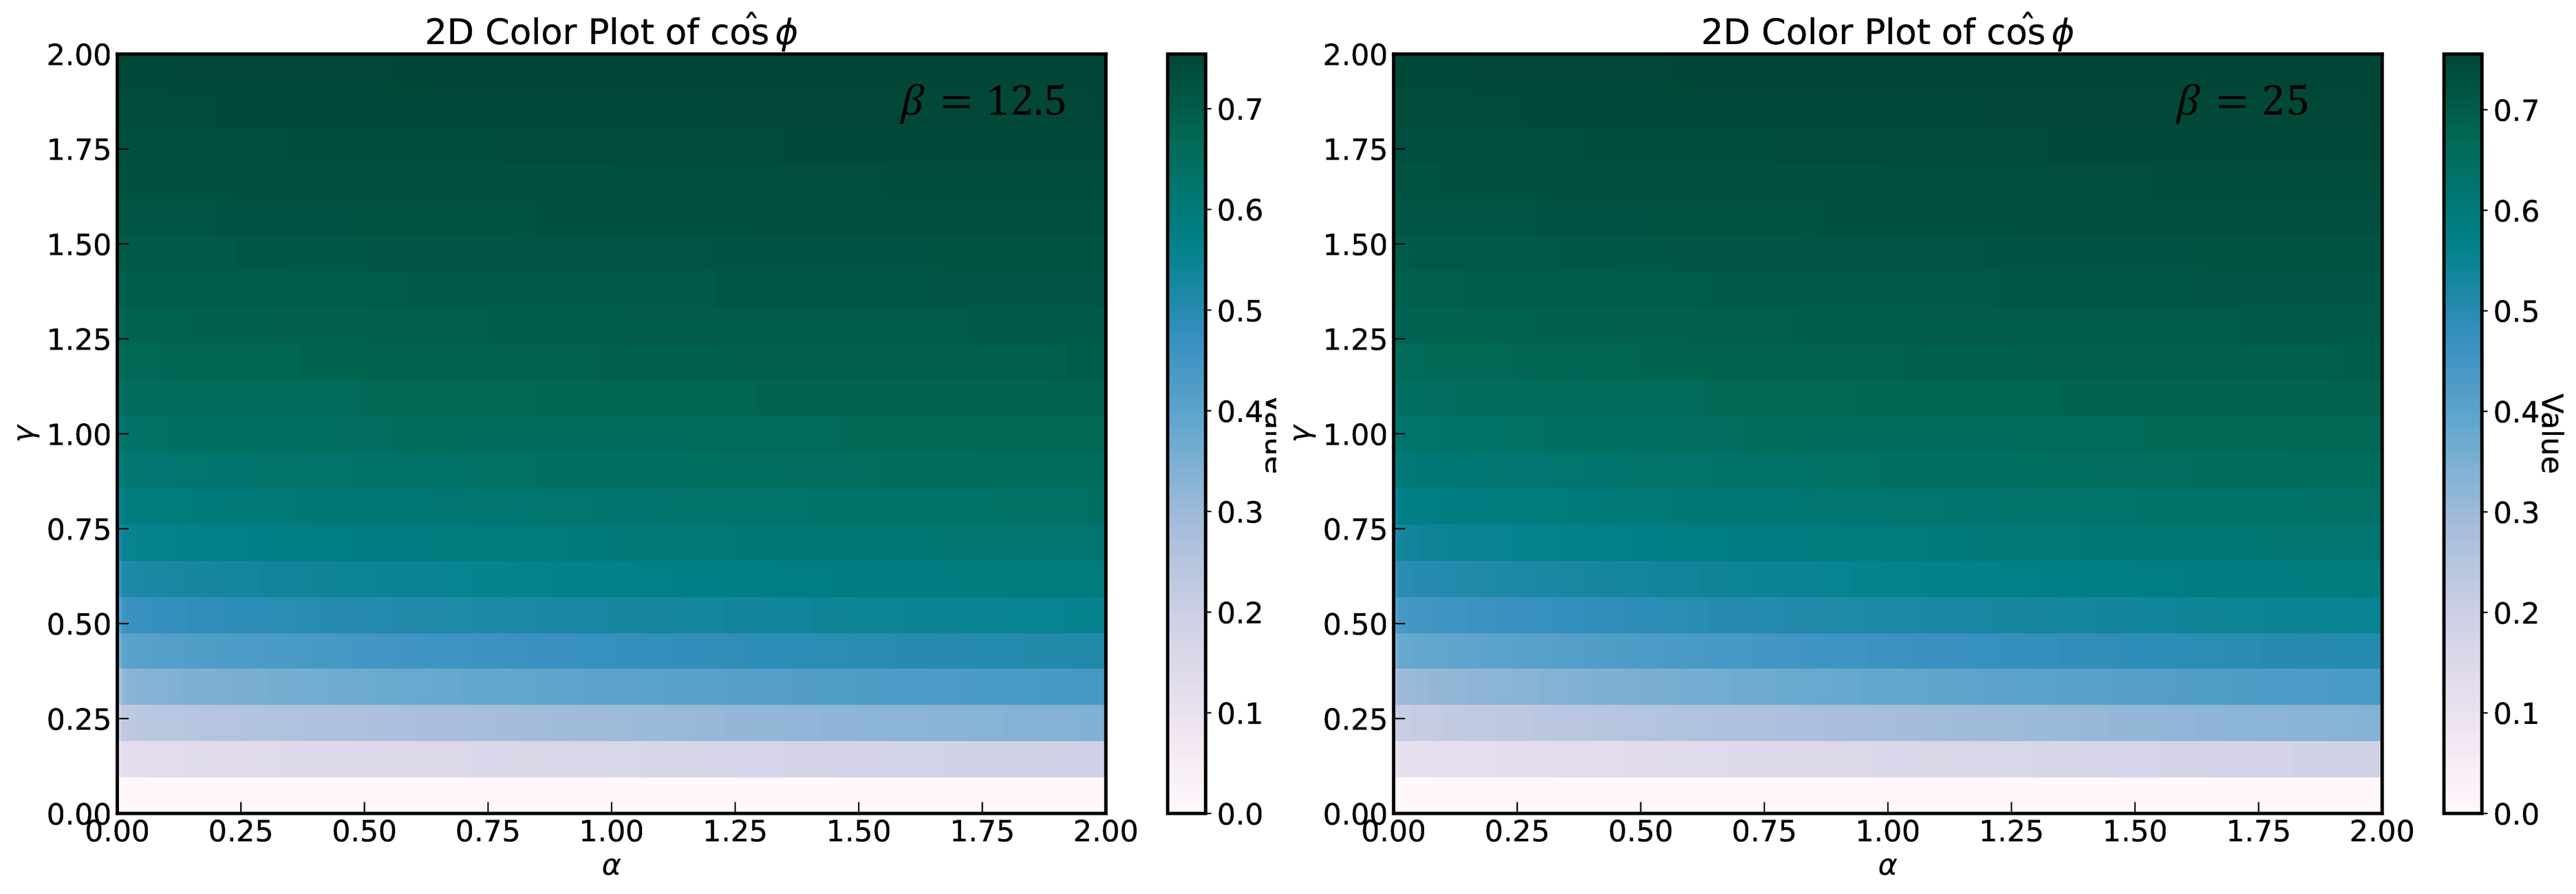
\includegraphics[width=16cm]{TexFigure/Order_color.png}}
  \caption{Colored plot for the expectation value of order parameter. The simulation was performed in NCA. The left figure is in the case of $\beta=10$, Right is for $\beta=25$.
  The difference in phase on each side of the junction goes lower as the color goes deeper.}
\end{figure}
\begin{figure}[htbp]
  \centerline{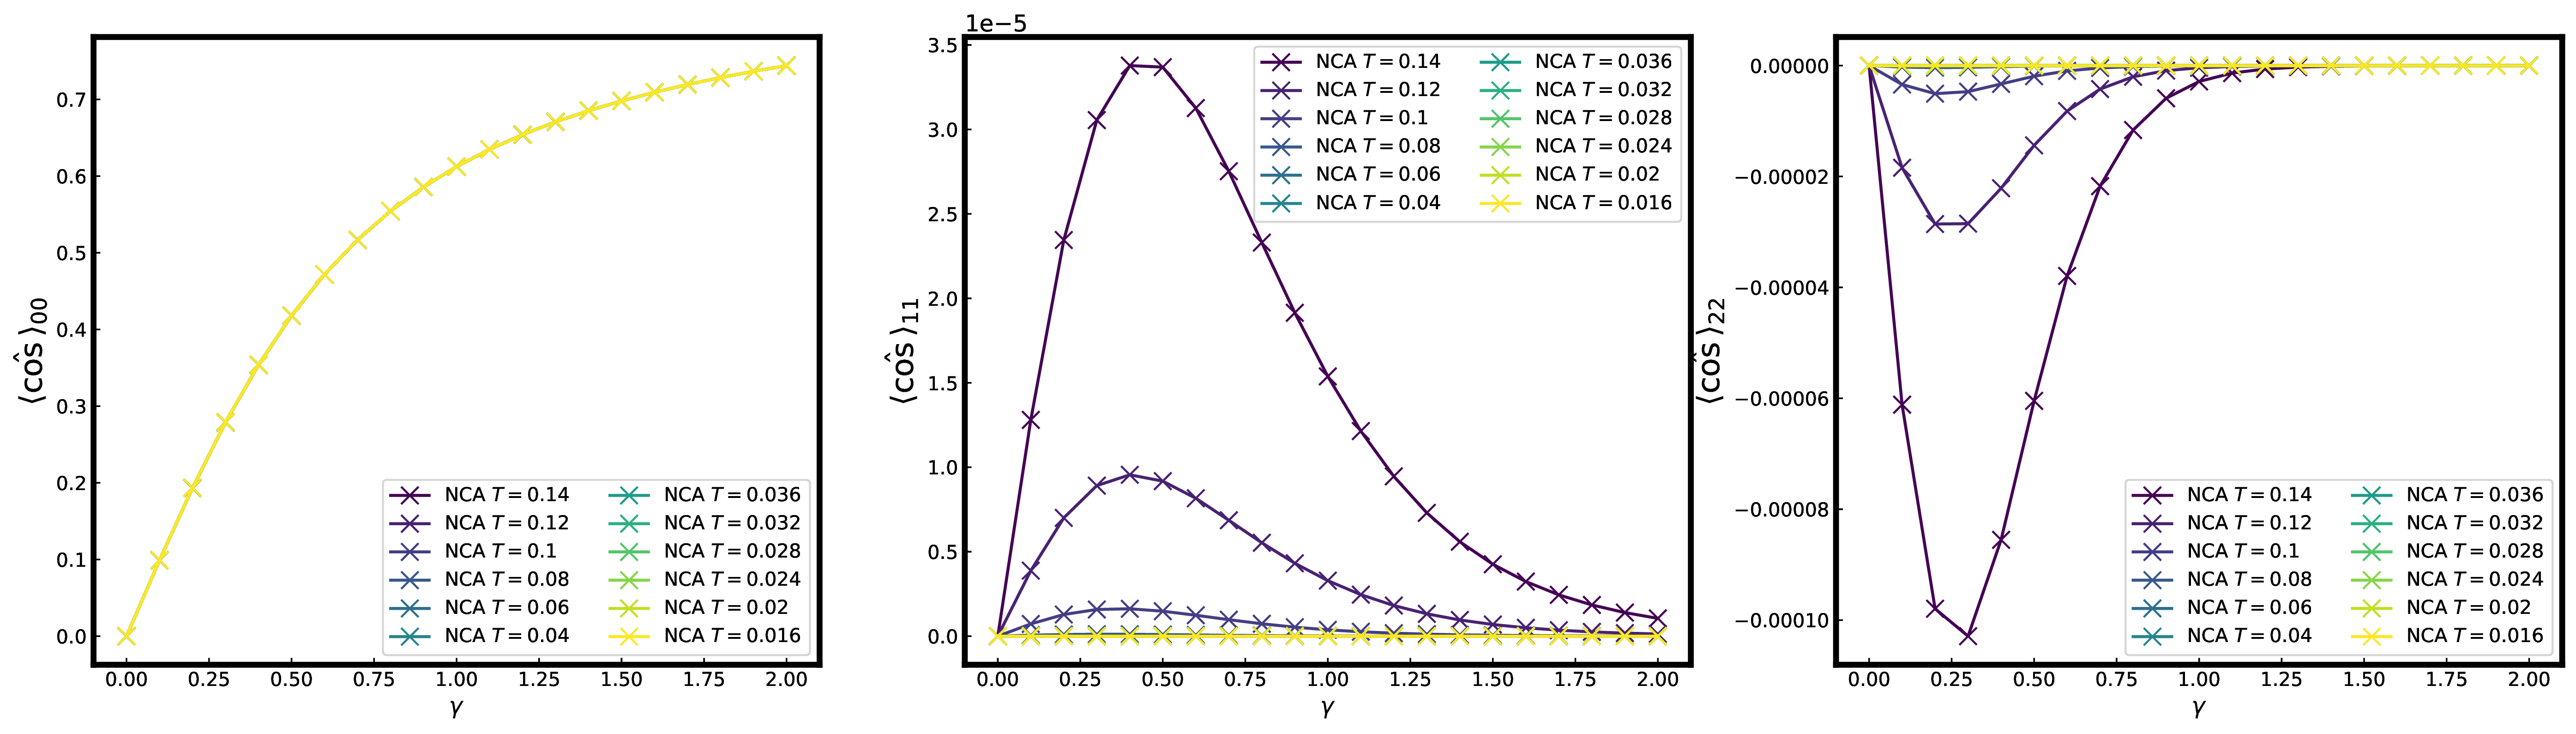
\includegraphics[width=17cm]{TexFigure/Matele_Ns3_alp0.png}}
  \centerline{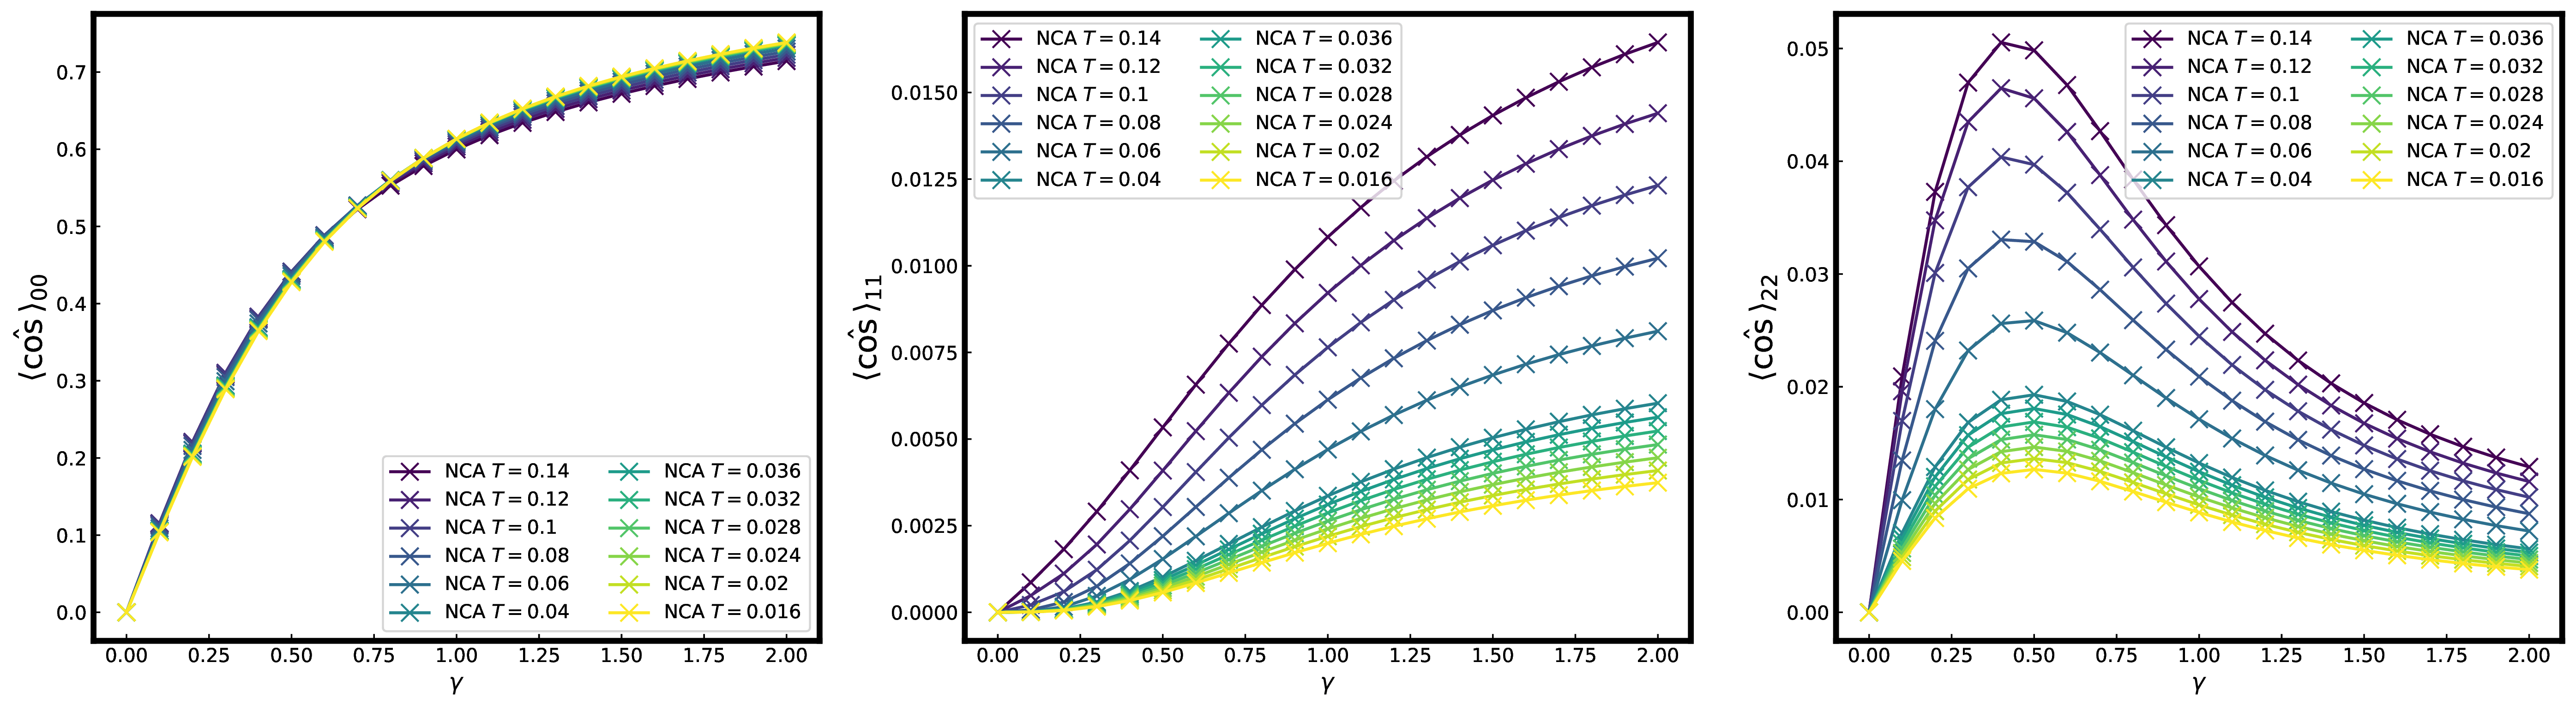
\includegraphics[width=17cm]{TexFigure/Matele_Ns3_alp0_1.png}}
  \centerline{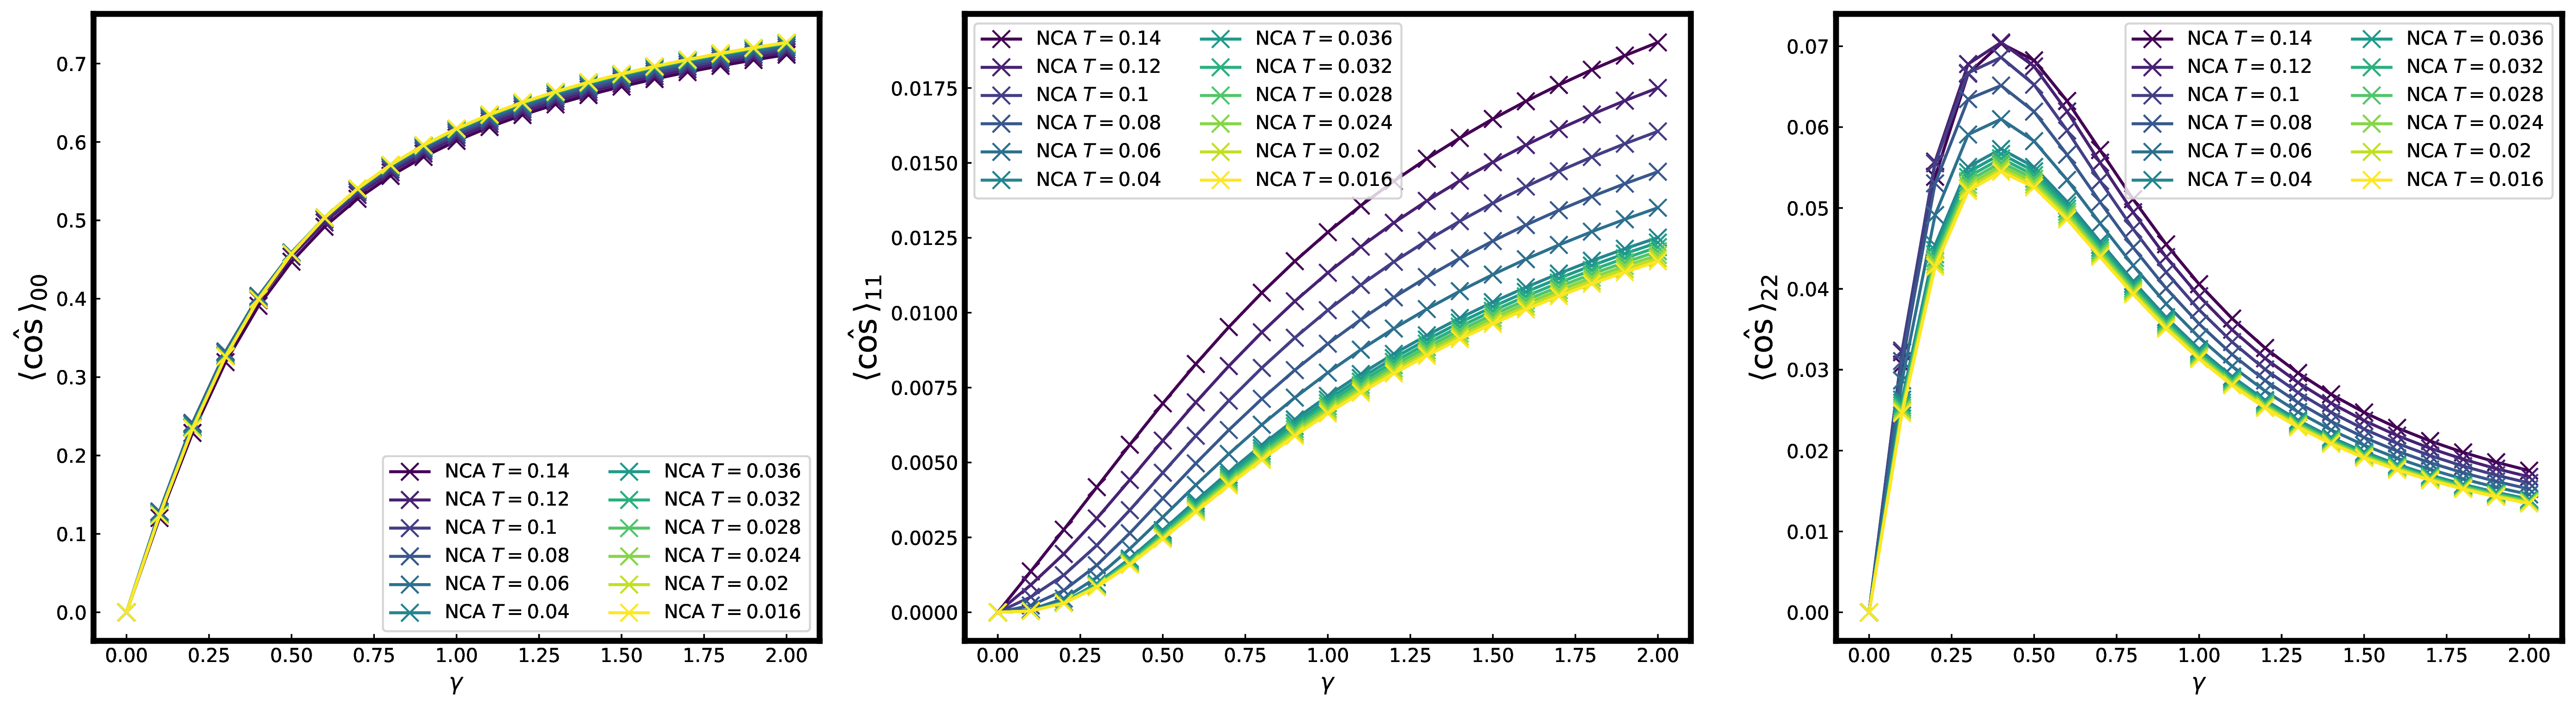
\includegraphics[width=17cm]{TexFigure/Matele_Ns3_alp1.png}}
  \caption{Plotting results of the diagonal elements of the product of the $\hat{\cos\phi}$ operator and the  
  $e^{H_{loc}}$ operator for different $\alpha$ values. From top to bottom, the results are for $\alpha$ 
  values of 0, 0.01, and 0.1, respectively. The first diagonal element is proportional to the probability of 
  the system being in the ground state, can be seen that it has the largest value among the diagonal elements 
  for all $\alpha $and $\gamma$ values. This confirms that the system tends to superconductivity regardless of 
  adjusting parameters.}
\end{figure}
\pagebreak
\subsubsection*{Temperature dependent transition}
To determine the criticality of the system's phase with respect to temperature, 
a new order parameter $\nu(T,\alpha,\gamma)$ was introduced, its change with respect to temperature was defined as follows:
\begin{flalign}
  \begin{split}
\frac{\partial \nu}{\partial T} \approx \frac{ \langle\hat{\cos \phi}\rangle|_{T_i} - \langle\hat{\cos \phi}\rangle|_{T_{i+1}}}{\Delta T} \quad , \quad \Delta T = |T_{i}-T_{i+1}|
\end{split}
\end{flalign}
Following the equation above, we observed the changes in the order parameter while varying the temperature. As the temperature decreases, the tangent of the orderparameter changes from a high slope to a low slope. This allows us to predict the temperature-dependent behavior of the system under investigation. The prediction of the system's phase change according to $\frac{\partial \nu}{\partial T}$ is follows:
\begin{flalign}
\begin{split}
\begin{cases}\frac{\partial \nu}{\partial T} > 0 \quad : \quad \text{Insulating} \\ \frac{\partial \nu}{\partial T} < 0 \quad : \quad \text{Superconducting}\\
\frac{\partial \nu}{\partial T} =0 \quad : \quad \text{crossover point}\end{cases}
\end{split}
\end{flalign}
When the simulation results were plotted on the $\alpha − \gamma$ plane, following three features were observed :\\
\indent - $\alpha$=0 (no interaction with the external reservoir), the system exhibits superconducting properties.\\
\indent - Crossover points on the $\alpha −\gamma$ plane for each consecutive temperature range, the left side of crossover line predicted as insulating properties and superconducting properties for right side.\\
\indent - As the temperature decreases, the range exhibiting insulating properties widens for a given $\alpha$ interval.\\
\begin{figure}[H]
  \centerline{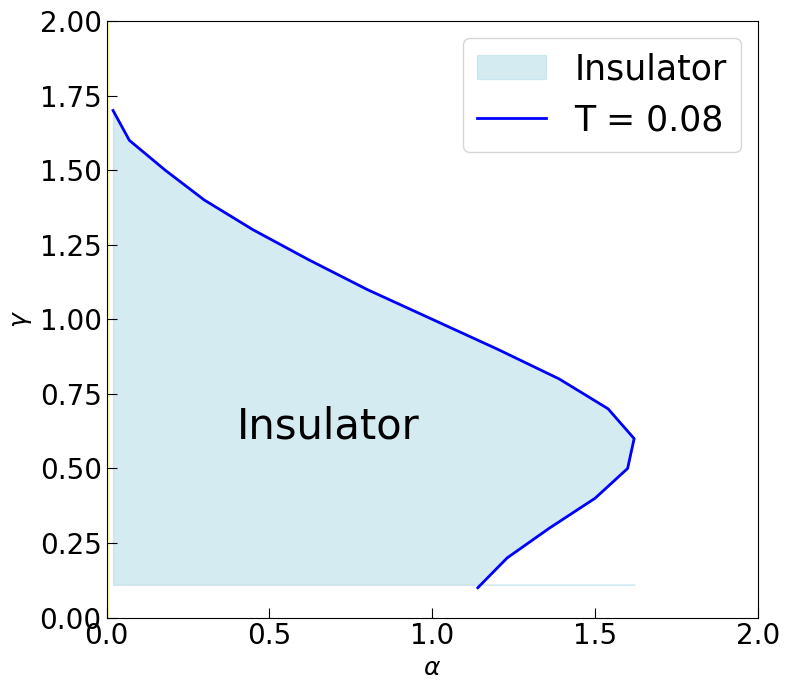
\includegraphics[width=8cm]{TexFigure/Simplefig.png}}
  \caption{Crossover tendency in $\alpha$ - $\gamma$ plane.}
\end{figure}
\pagebreak
\newpage
\begin{figure}[H]
  \centerline{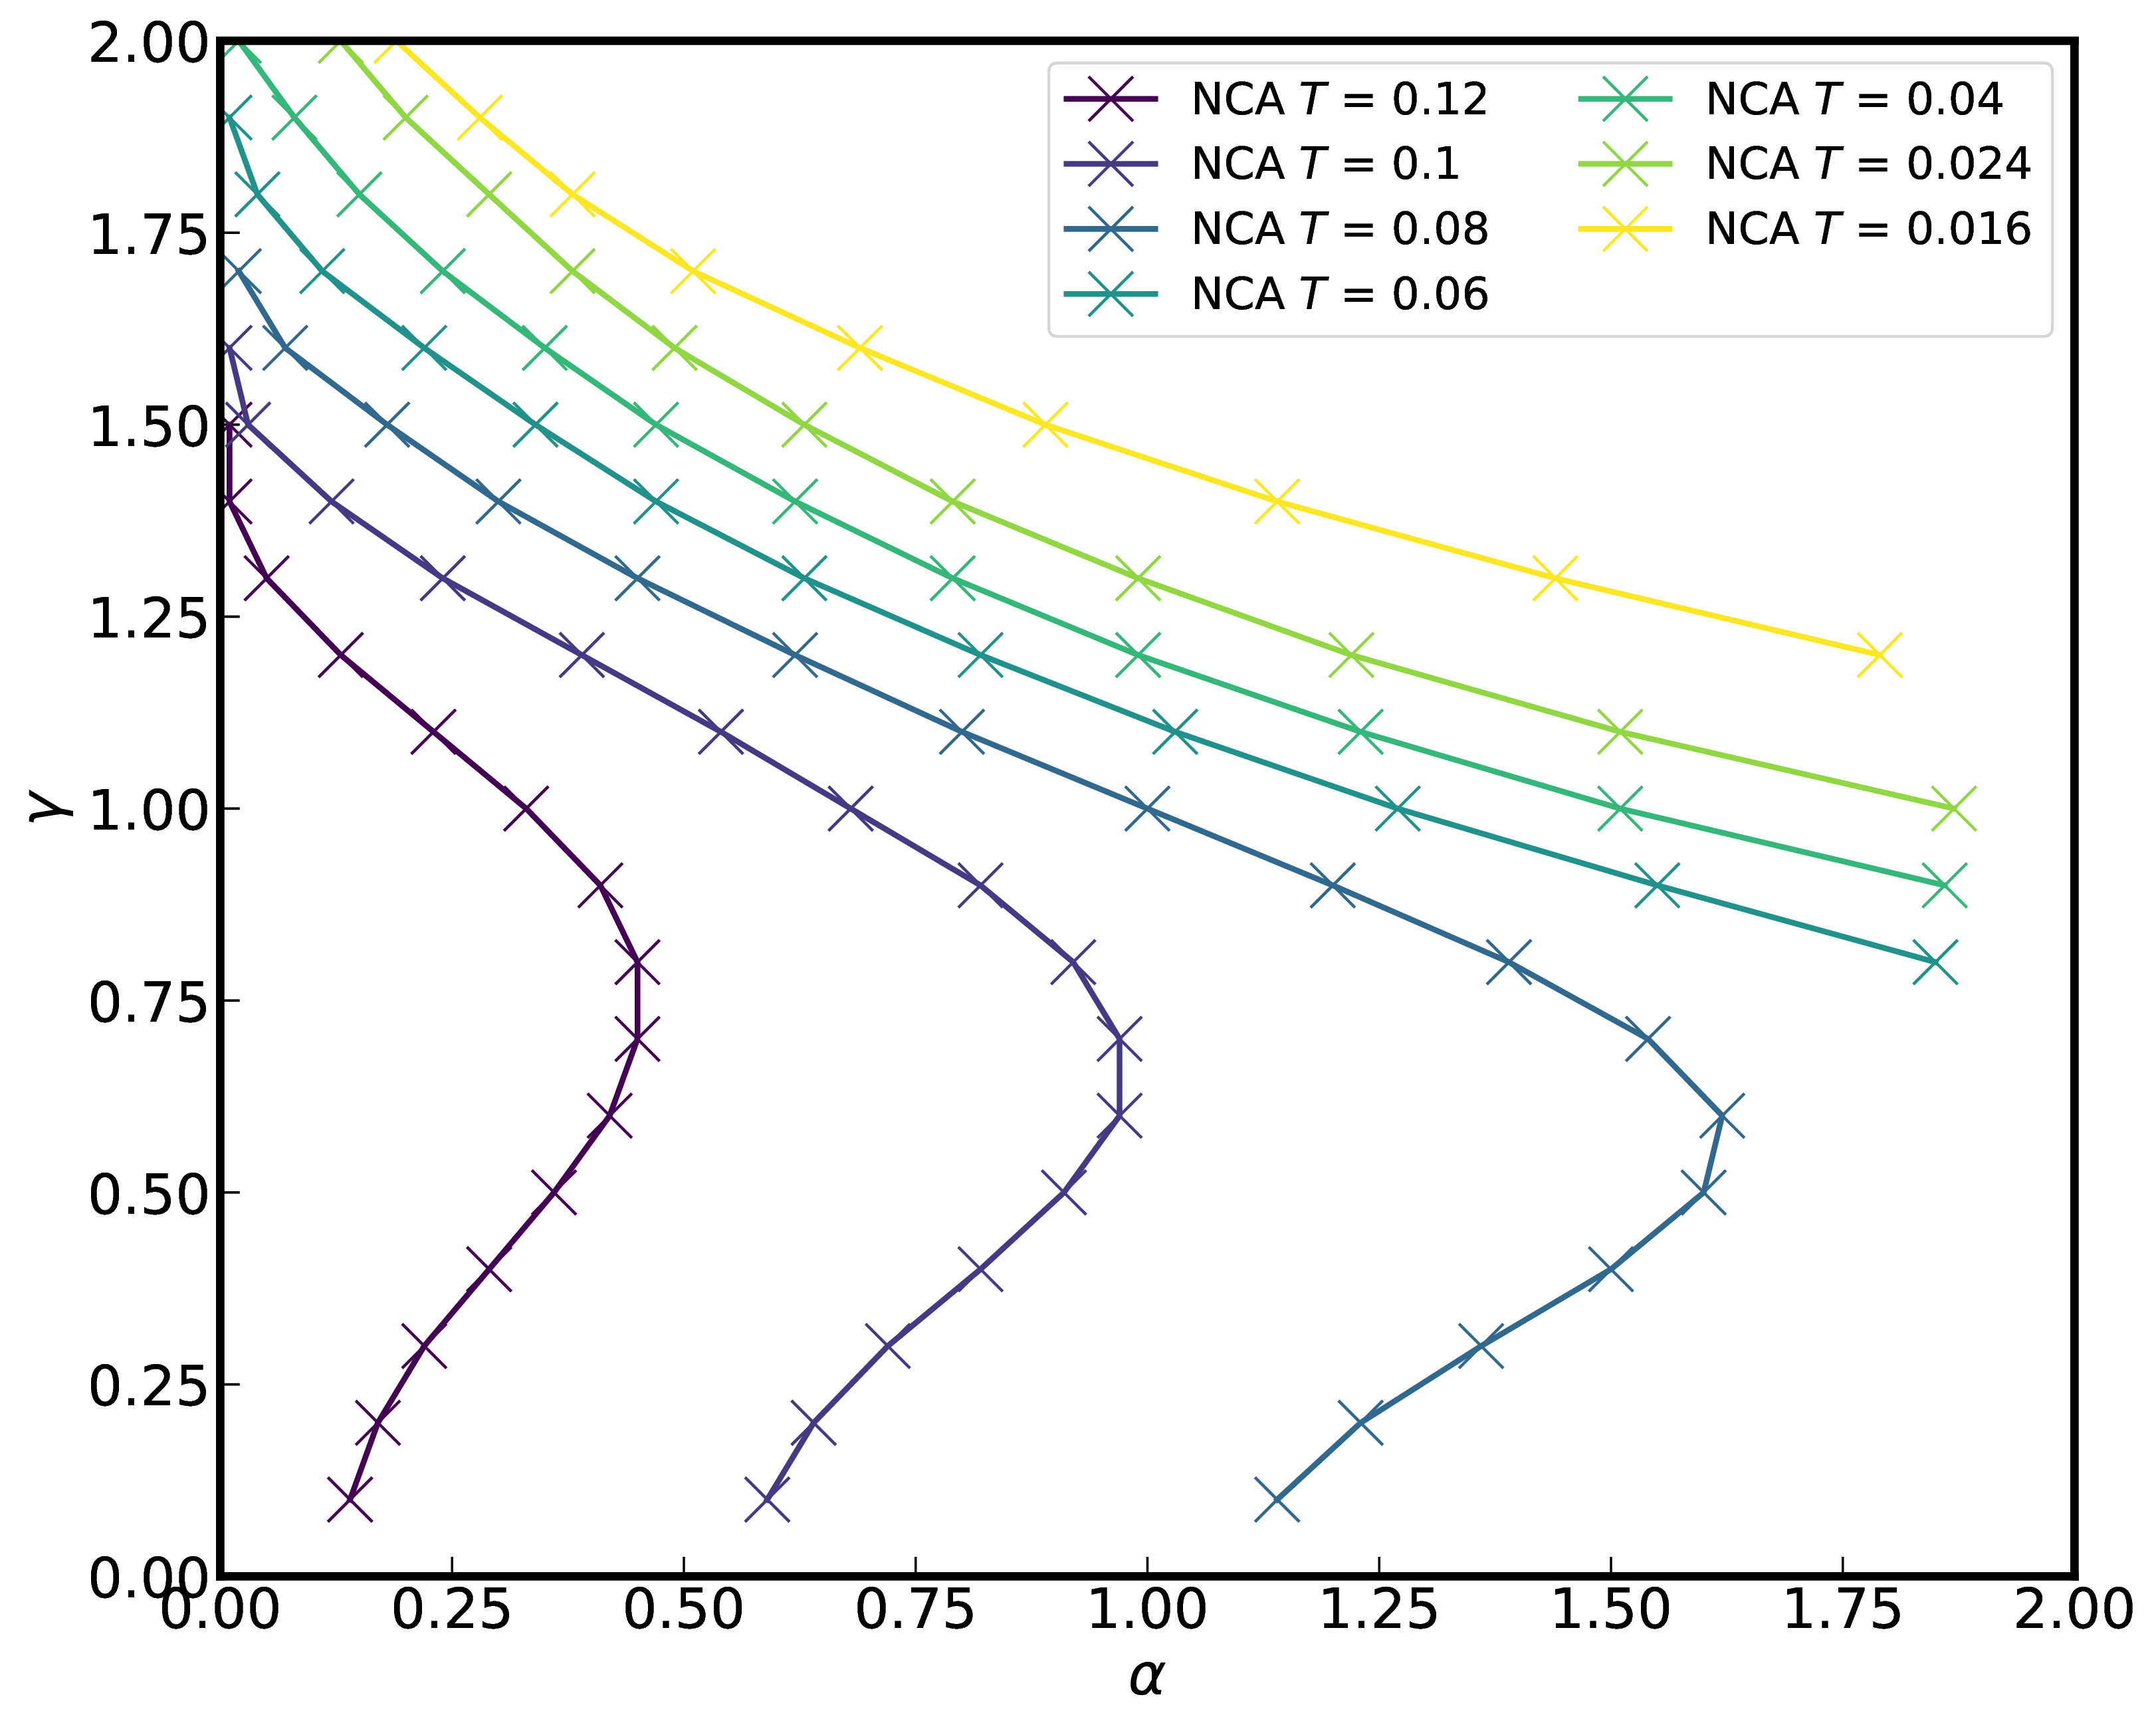
\includegraphics[width=12cm]{TexFigure/3dplot_Ns3_proj_n-1.png}}
  \centerline{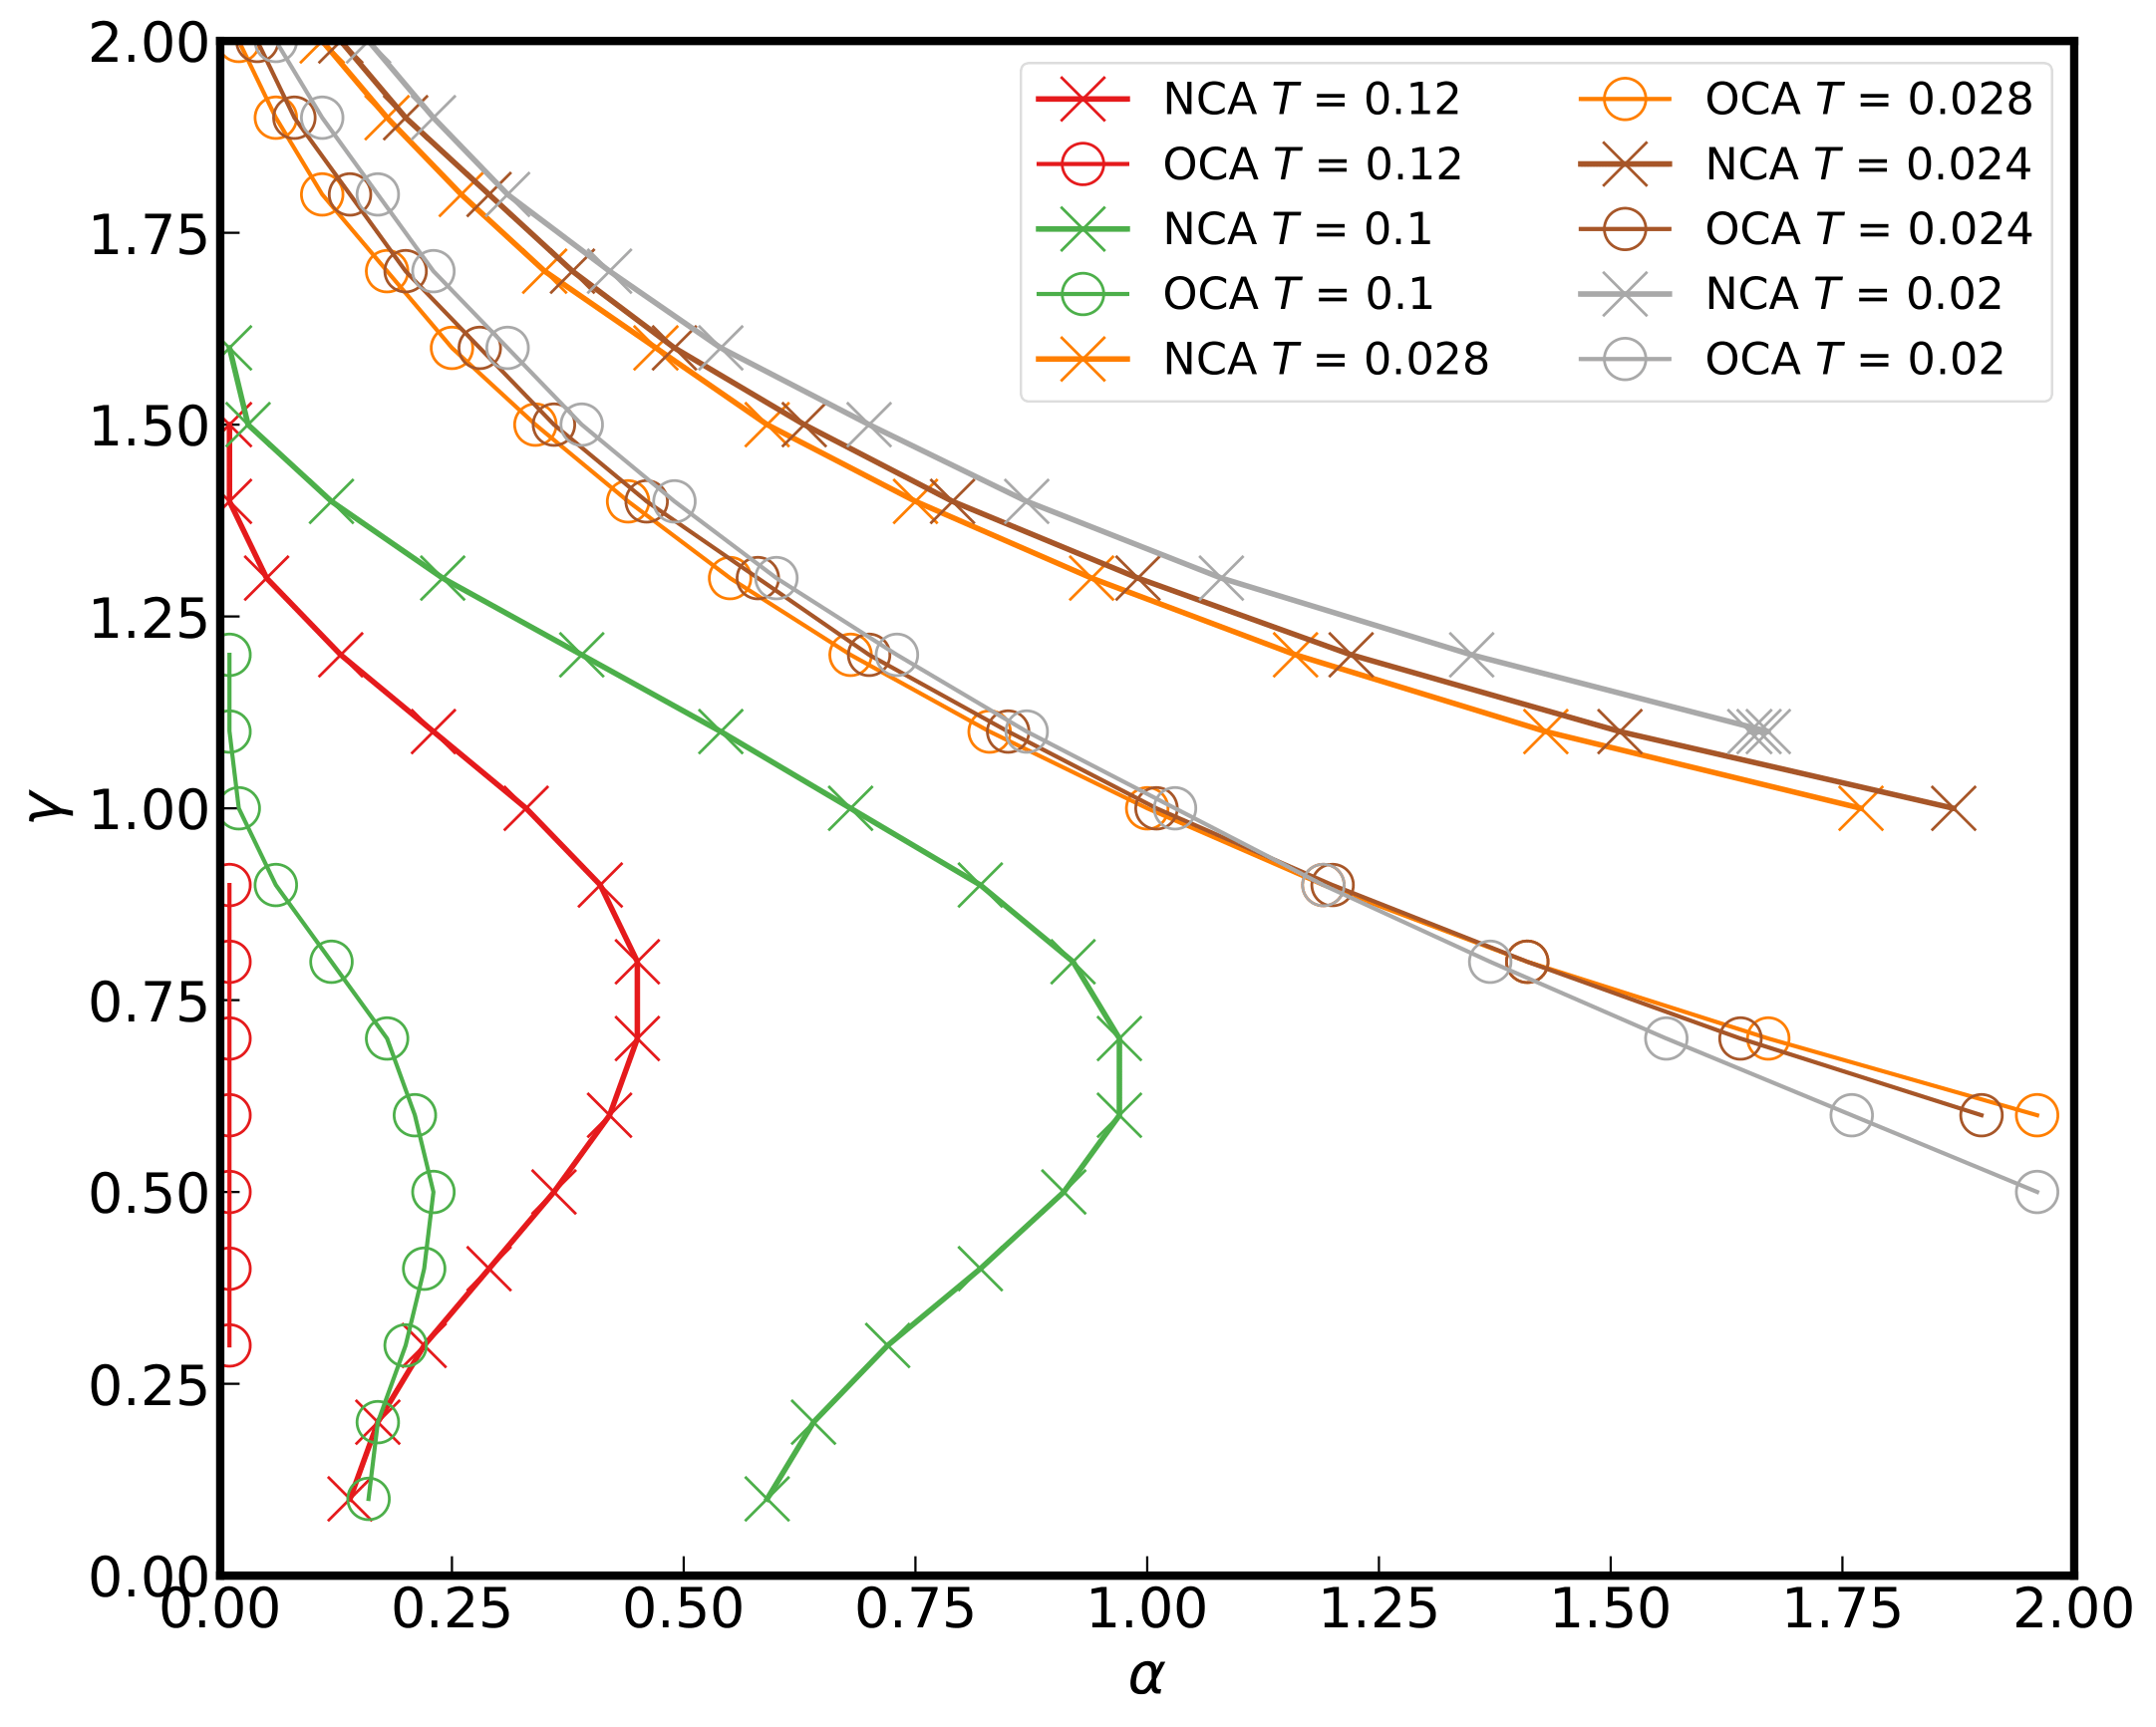
\includegraphics[width=12cm]{TexFigure/3dplot_COMP3_proj_n-1.png}}
  \caption{The points indicate where the abrupt change of the order parameter $\nu$ with temperature difference. 
  Notated temperature is the lower value of the two consecutive temperature values 
  (e.g., T = 0.12 represents the line connecting the points where the difference of $\nu$ values 
  for the two temperatures [0.1, 0.12] becomes 0). The upper plot shows the results calculated using NCA, 
  and the lower plot compares the results of OCA and NCA under the same temperature condition.}
  \label{2Dplot}
\end{figure}
\begin{figure}[H]
  \centerline{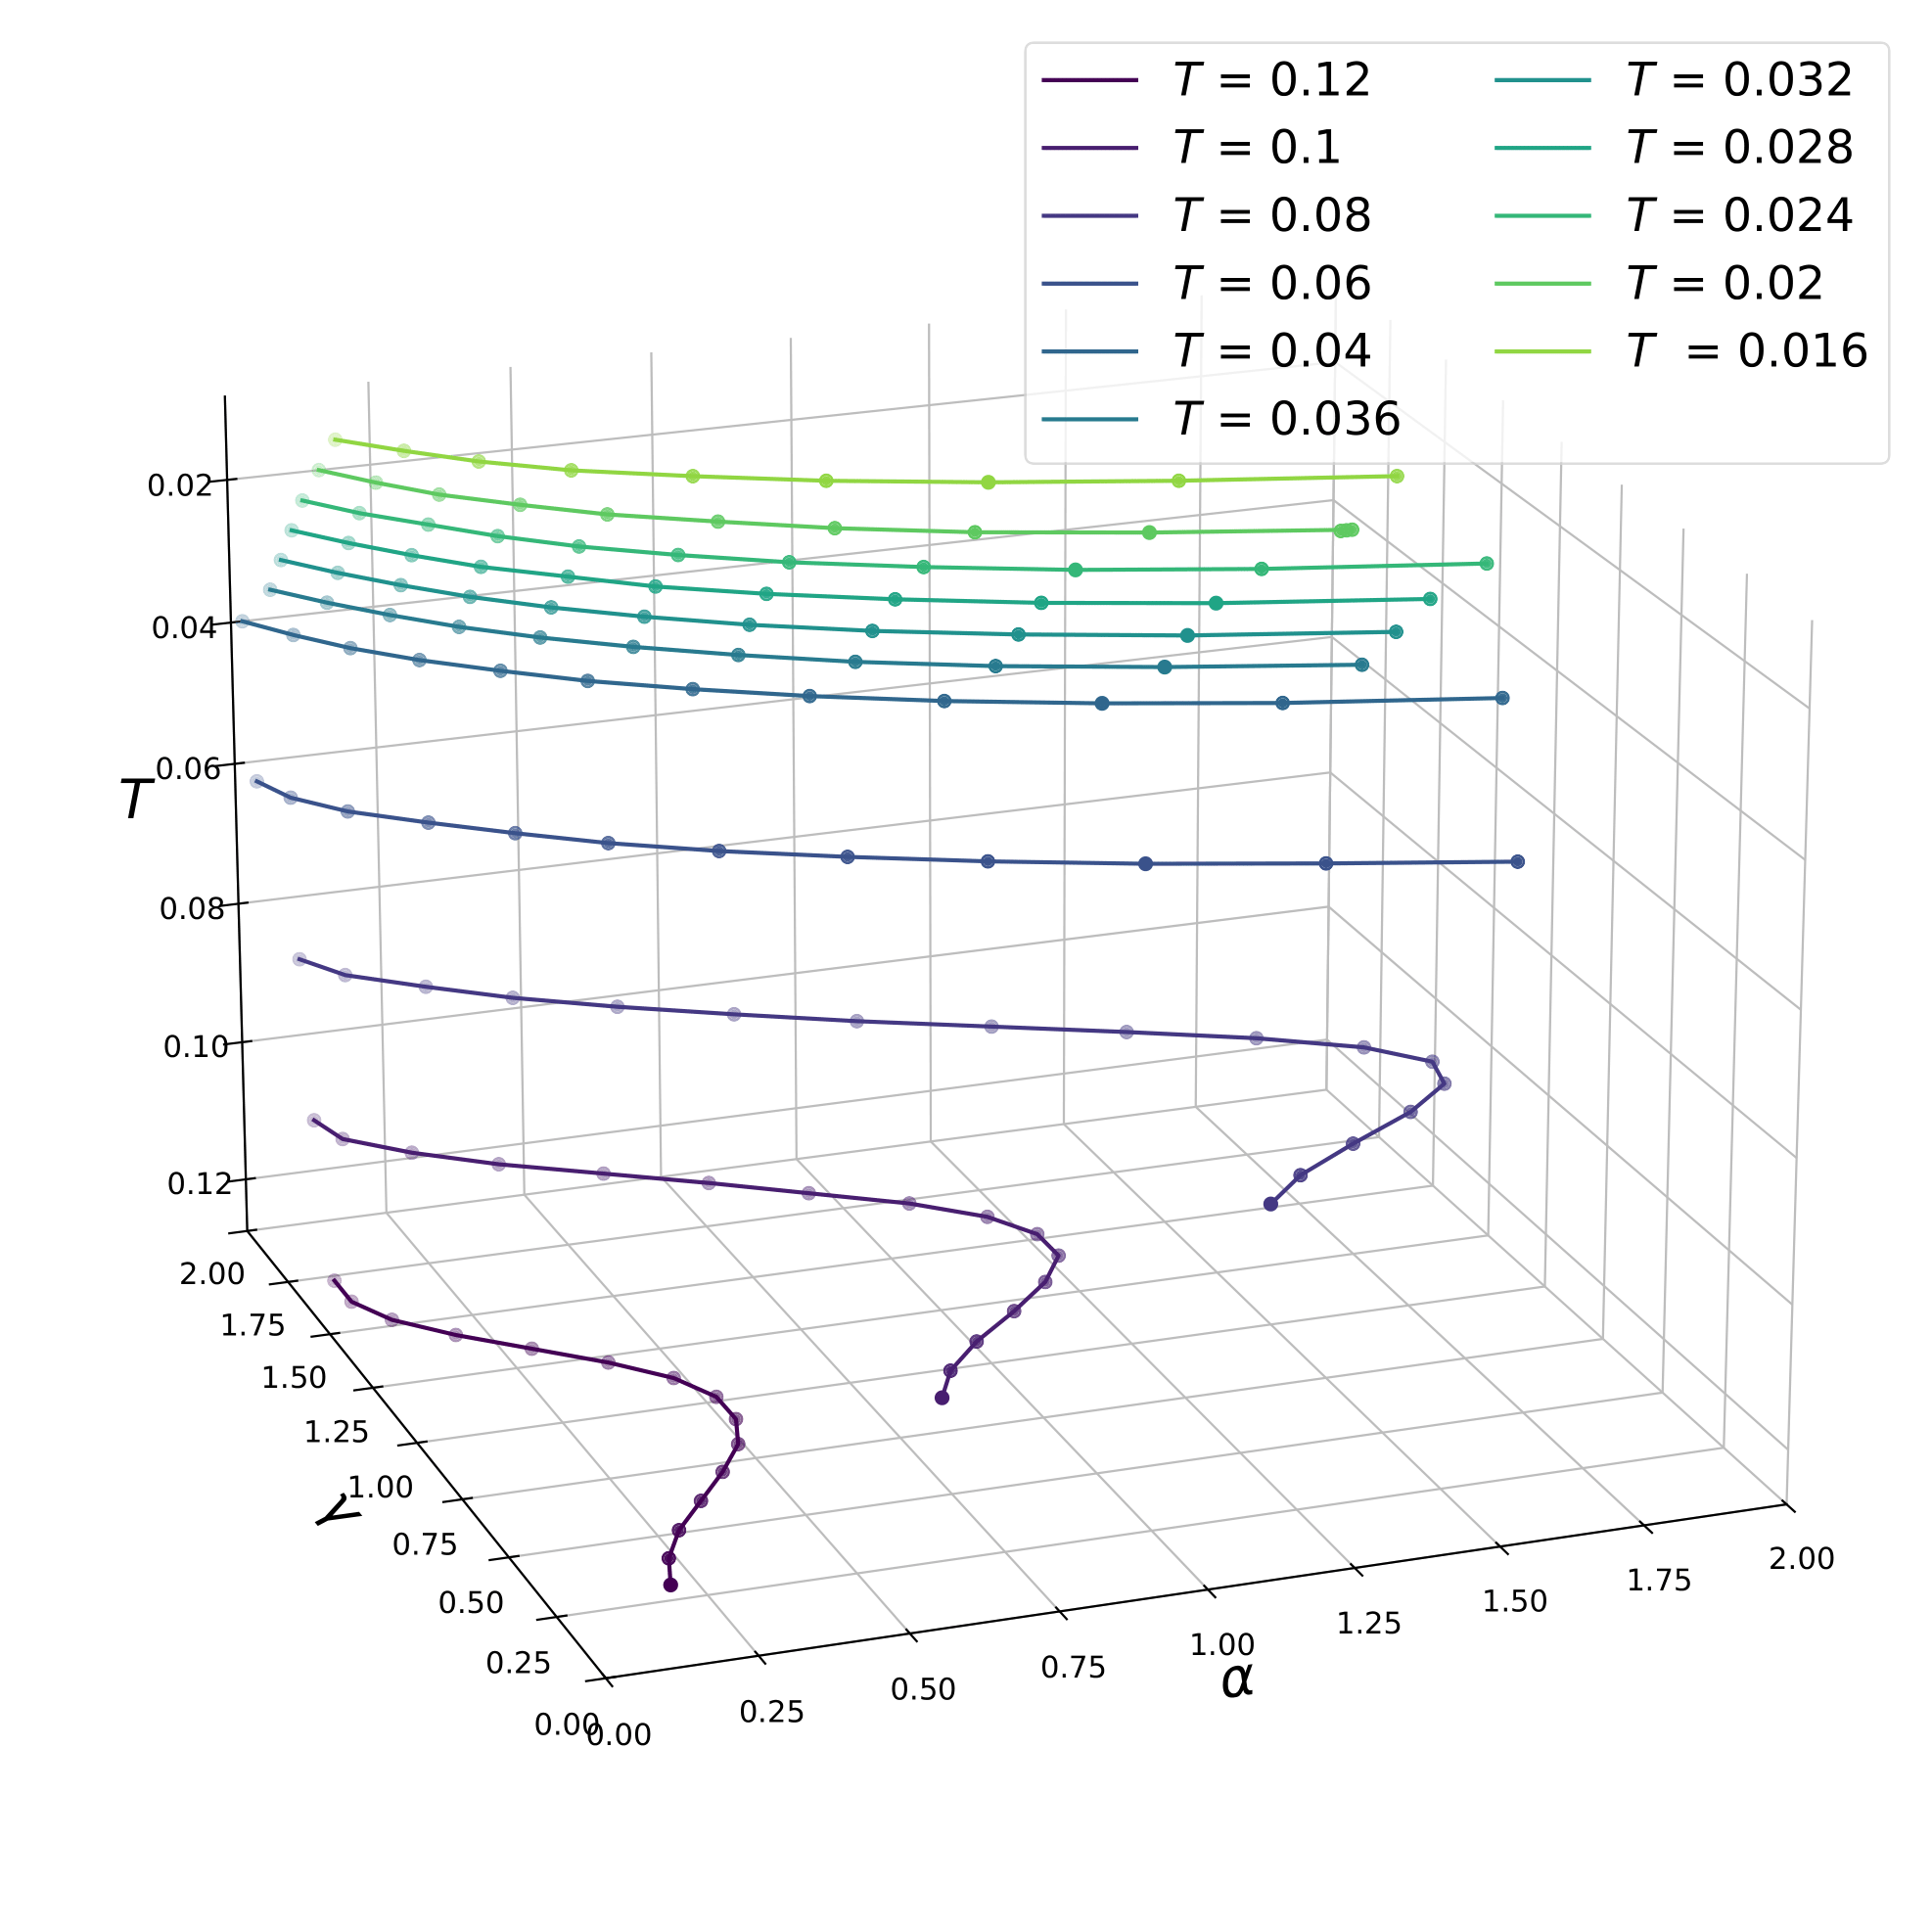
\includegraphics[width=17cm]{TexFigure/3dplot_Ns3_proj_20-1.png}}
  \caption{3-Dimension plotting of upper Figure 23, with $T$ axis}%\ref{2Dplot}%,  with $\beta$ axis}
\end{figure}
\pagebreak
\begin{figure}[H]
  \vfill
  \centering
  \centerline{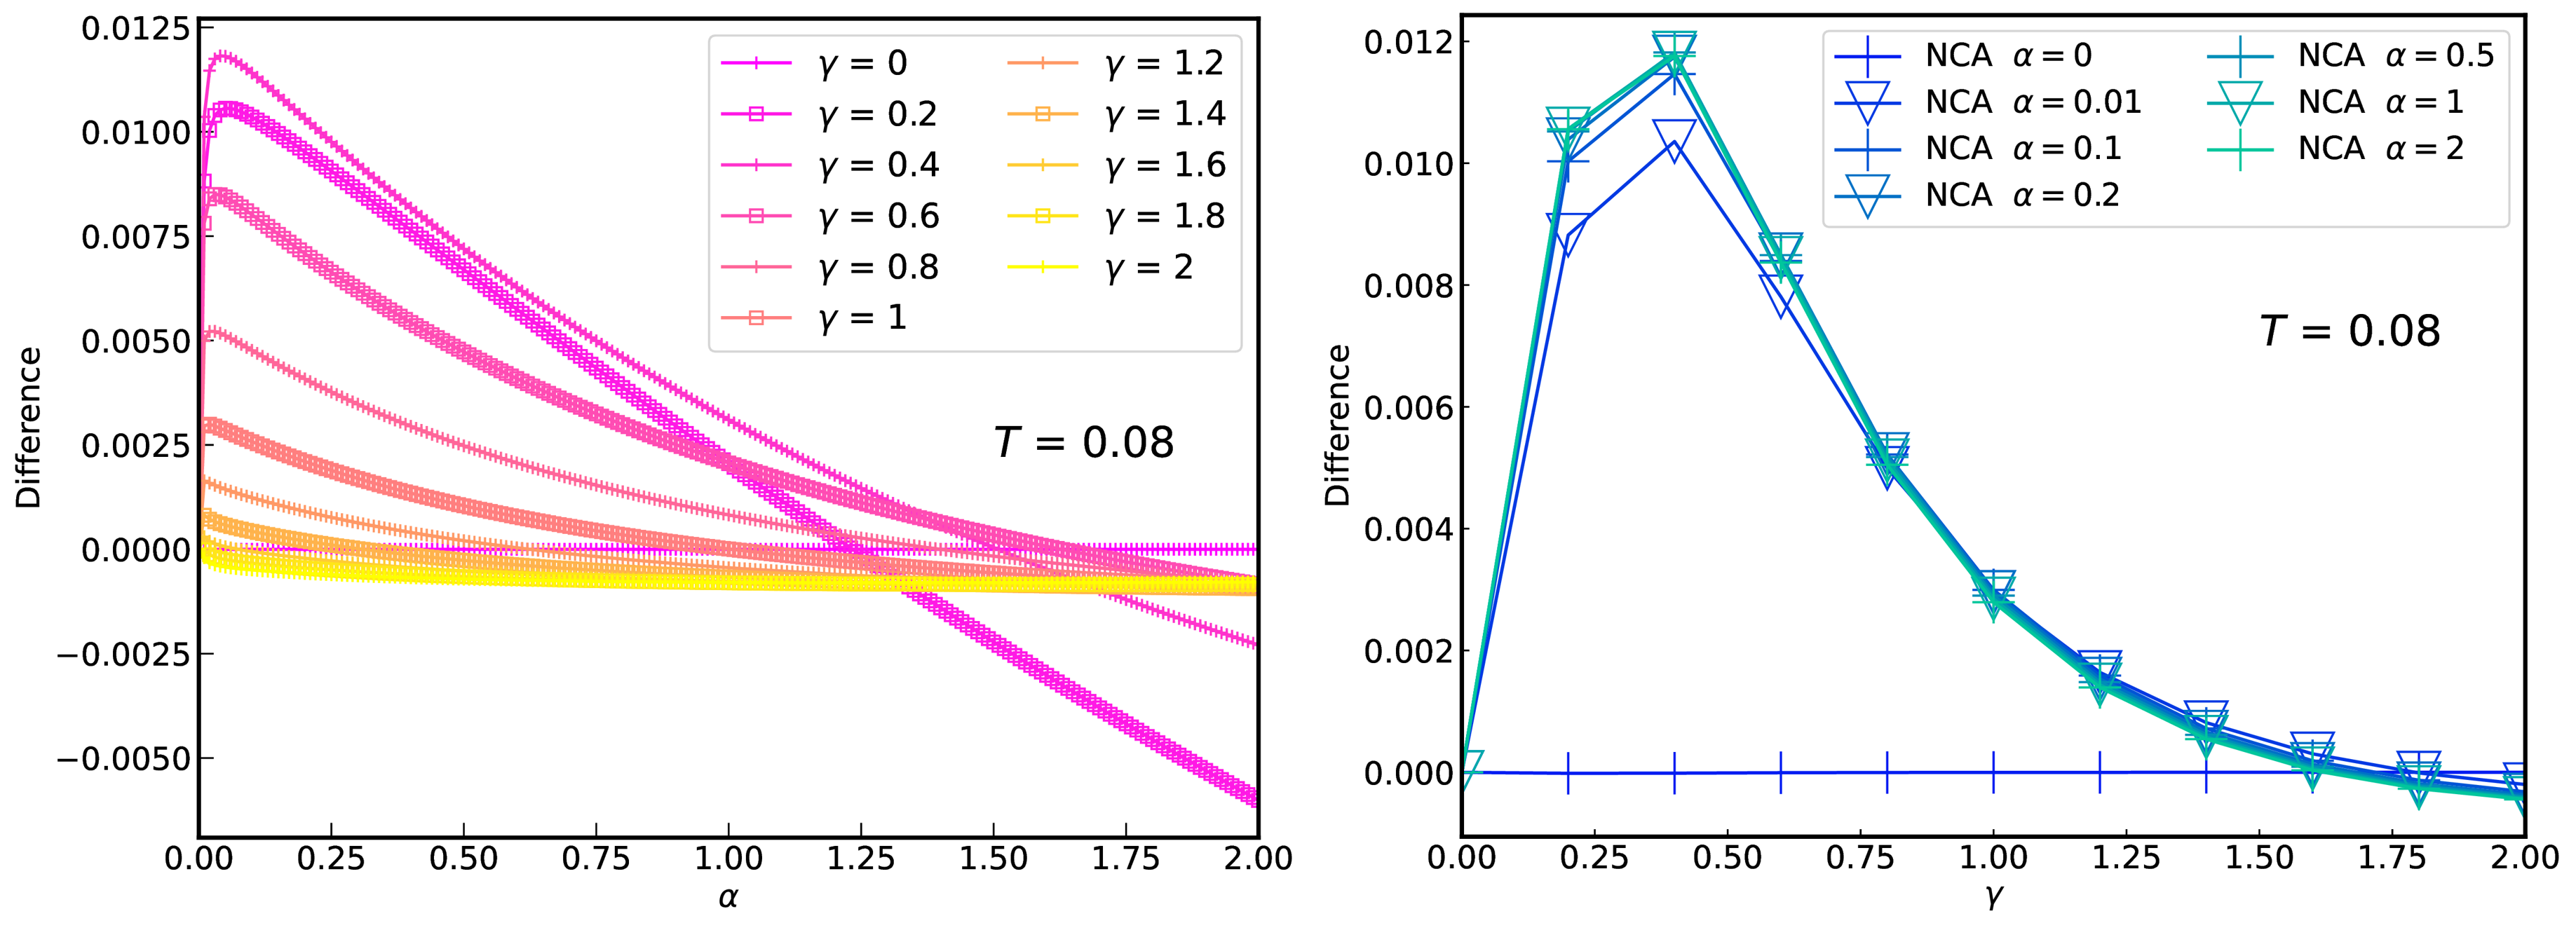
\includegraphics[width=17cm]{TexFigure/swap_fig.png}}
  \caption{Left : Crossover tendency for fixed $\gamma$ and $T$ with varying $\alpha$ value. Right : Crossover tendency for fixed $\alpha$ and $T$ with varying $\gamma$ value.}
\end{figure}
\begin{figure}[H]
  \vfill
  \centering
  \centerline{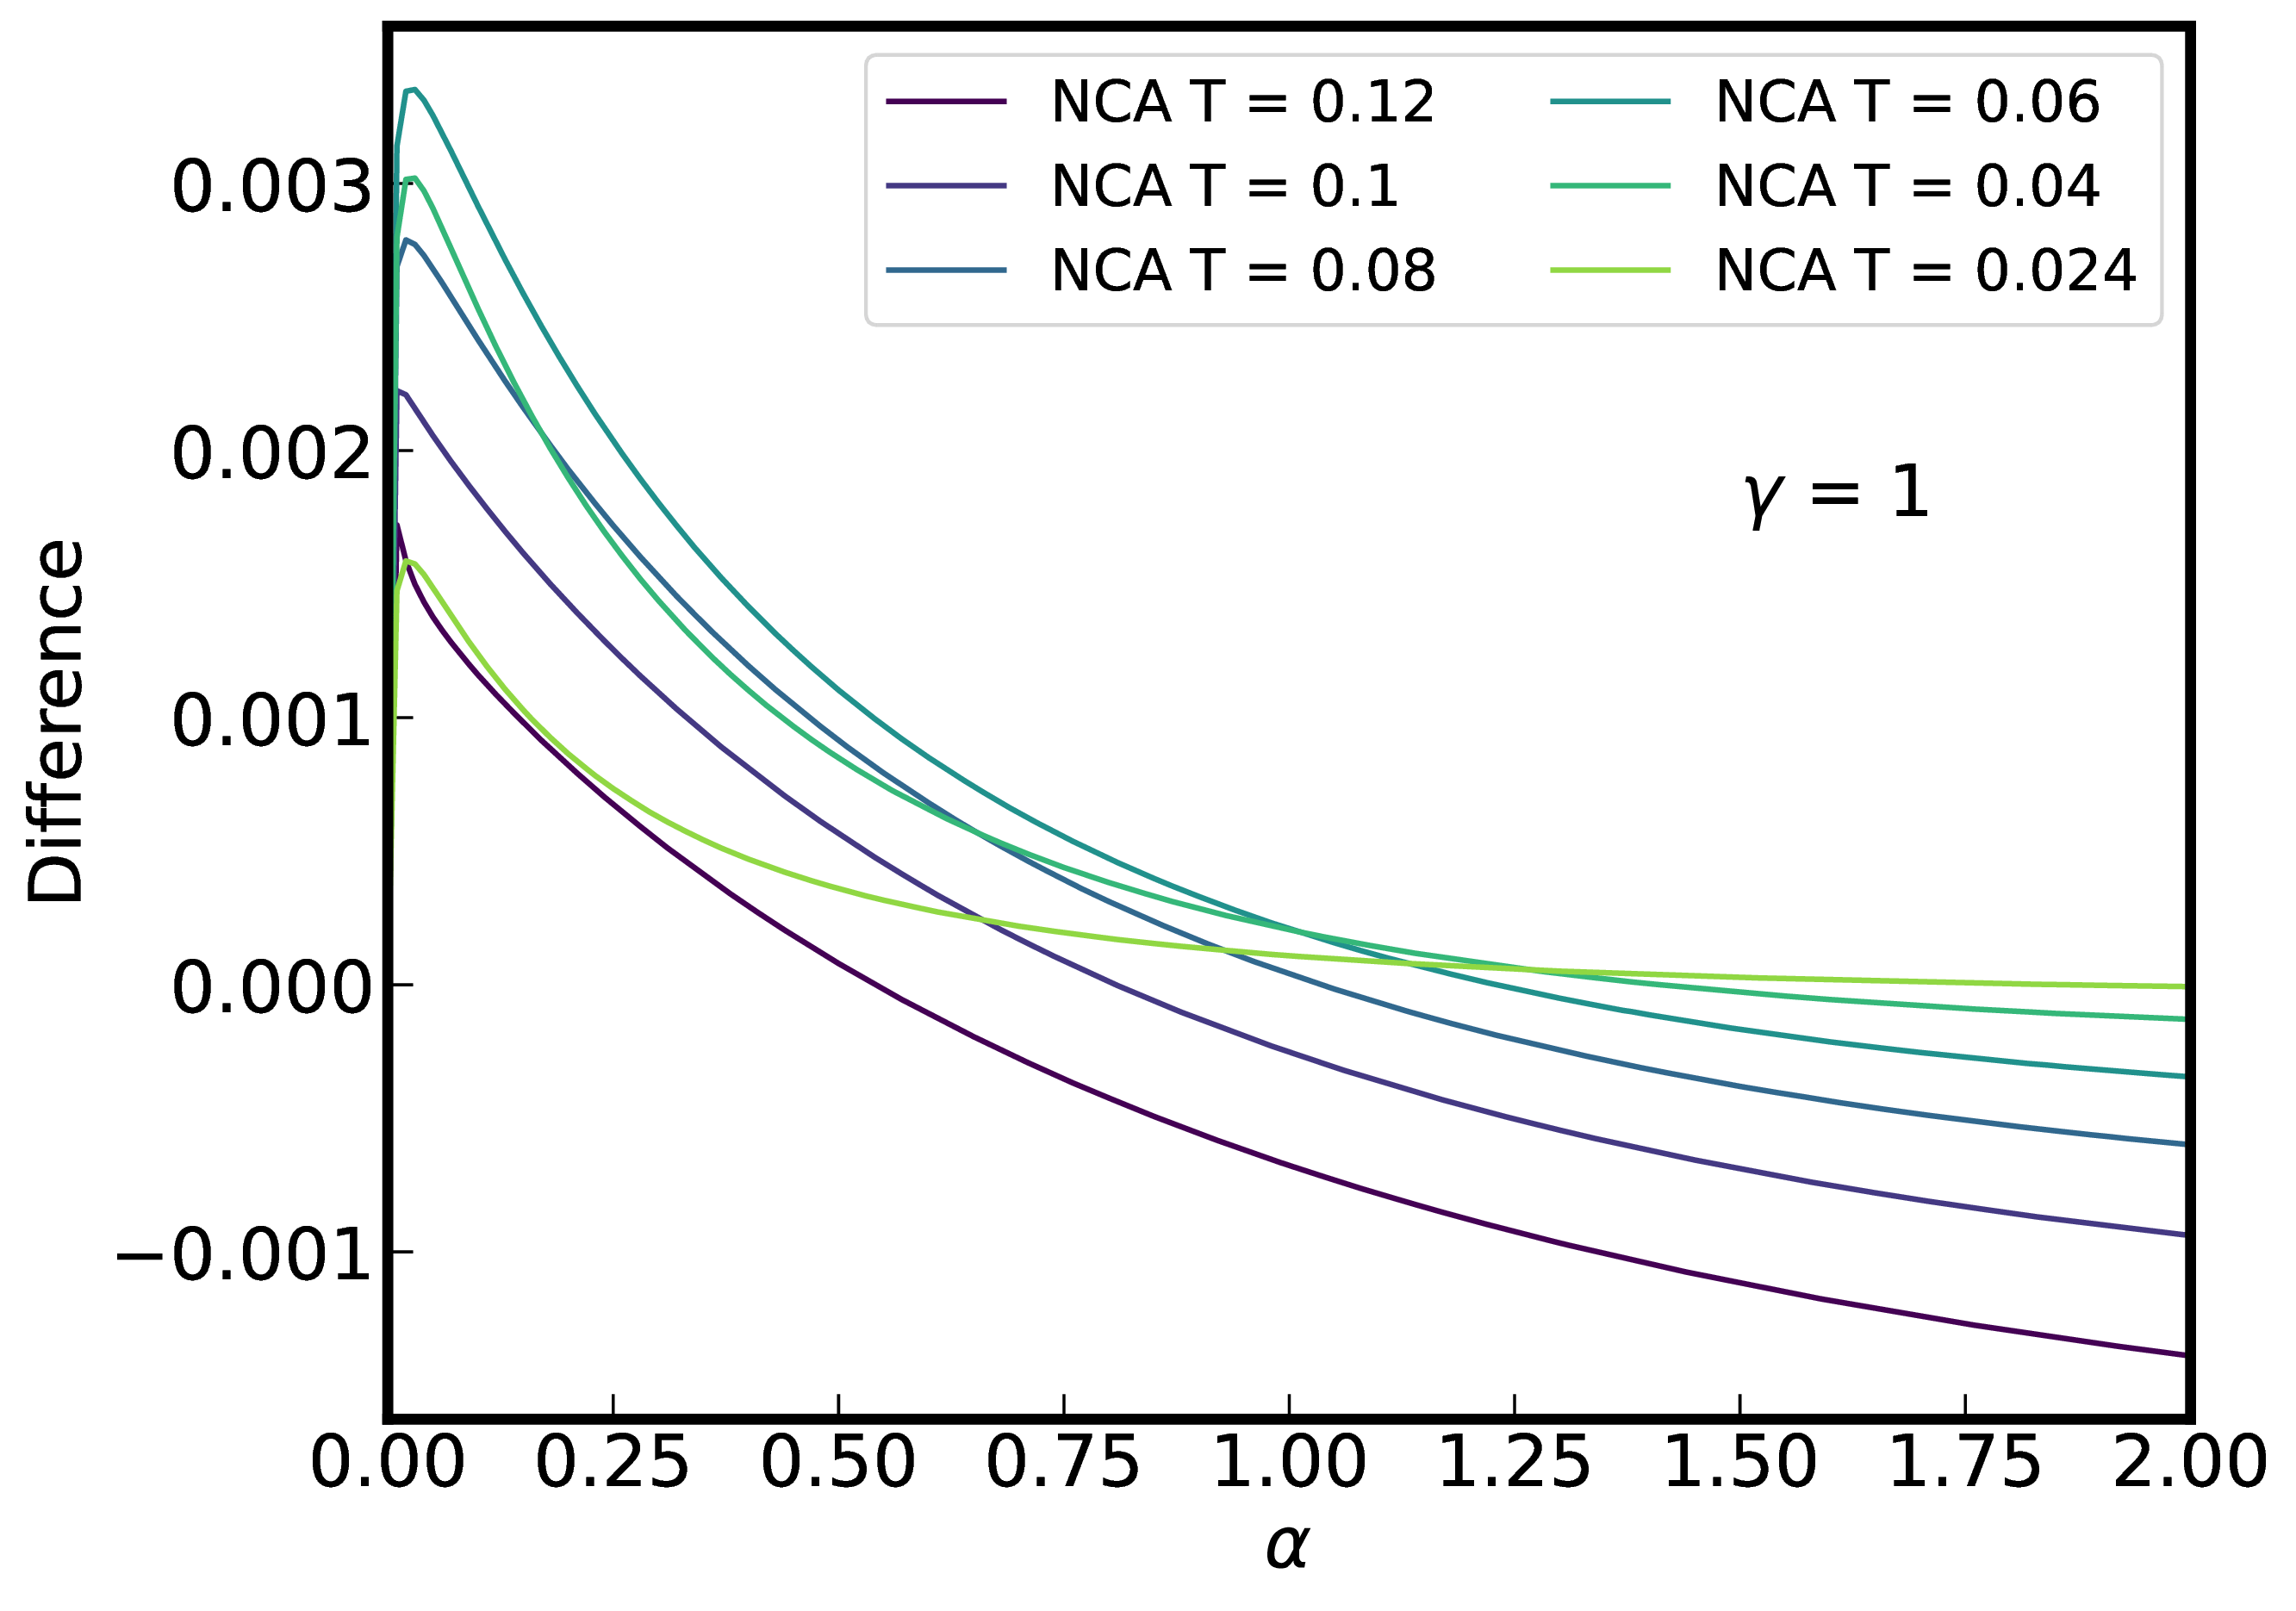
\includegraphics[width=12cm]{TexFigure/Diff_gam_1-1.png}}
  \caption{Crossover tendency for fixed $\gamma$ and $T$ with varying $\alpha$ value.}
\end{figure}

\newpage
\subsubsection*{Small alpha}
In the calculation of $\hat{\cos\phi}$ at the value from $\alpha$ = 0 to near a small value, 
the system change shows a discontinuous behavior from superconductor to insulator. 
According to the right side in Figure 17, 
  we can deduce two features:  \\
  \indent 1. when $\alpha=0$ there is no sign change in the order parameter,  \\
  \indent 2. the value of $\hat{\cos\phi}∣_{T_i}−\hat{\cos\phi}∣_T_{i+1}$ is always negative, 
  suggesting that system exhibits superconductivity as the temperature decreases. \\
  This contradicts the left side of the crossover line represents the insulator state. 
To investigate how the phase change of the junction varies when the influence of the external environment is small, 
we applied the approximation method in a small $\alpha$ interval. Updated alpha range follows:
\begin{table}[htbp]
  \centering
  \renewcommand{\arraystretch}{1.2}  % 행 간격 조정
  \begin{tabular}{@{}ccc@{}}
  \toprule
  \textbf{Previous $\alpha$} & \textbf{Updated $\alpha$} & \textbf{Interval}\\ 
  \midrule
  \text{[0,2]} & \text{[0,0.0001]} & 201 \\
  \bottomrule
  \end{tabular}
  \caption{Updated $\alpha$ range for simulation. Other conditions were left unchanged.}
  \end{table}

  The calculation results showed that the sign of $\frac{\partial \nu}{\partial T}$ changes from negative to positive 
as the $\gamma$ is varied within a specific temperature range. The existence of a continuous crossover from superconductor 
to insulator is presumed within a small $\alpha$ interval.
\begin{figure}[H]
  \centerline{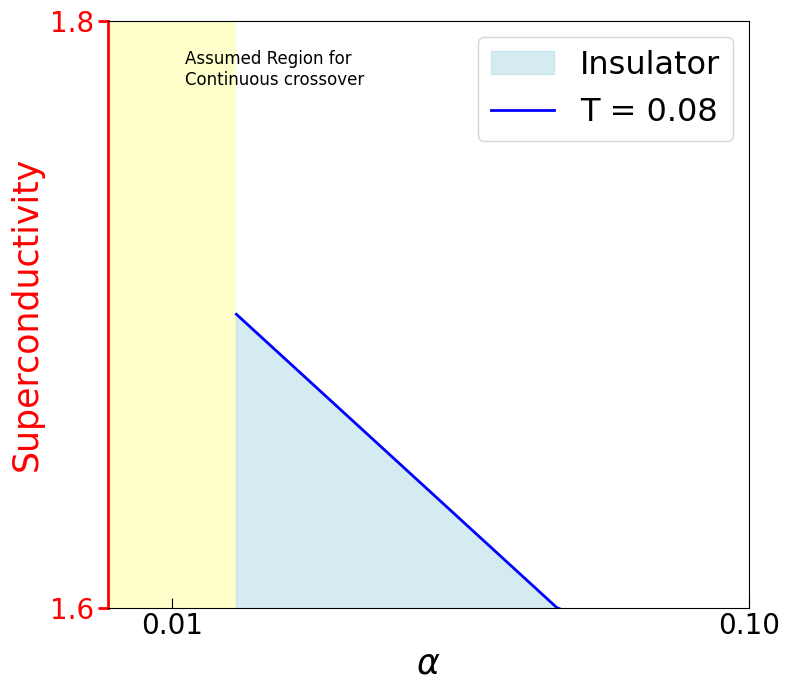
\includegraphics[width=8cm]{TexFigure/smallalp.png}}
  \caption{Expected temperature-dependent phase change behavior from the results.
  We can deduce that the system will show a continuity corresponding to the superconductor-to-insulator transition in the small $\alpha$ value interval.}
\end{figure}
\pagebreak
\vfill
\begin{figure}[H]
  \vfill
  \centerline{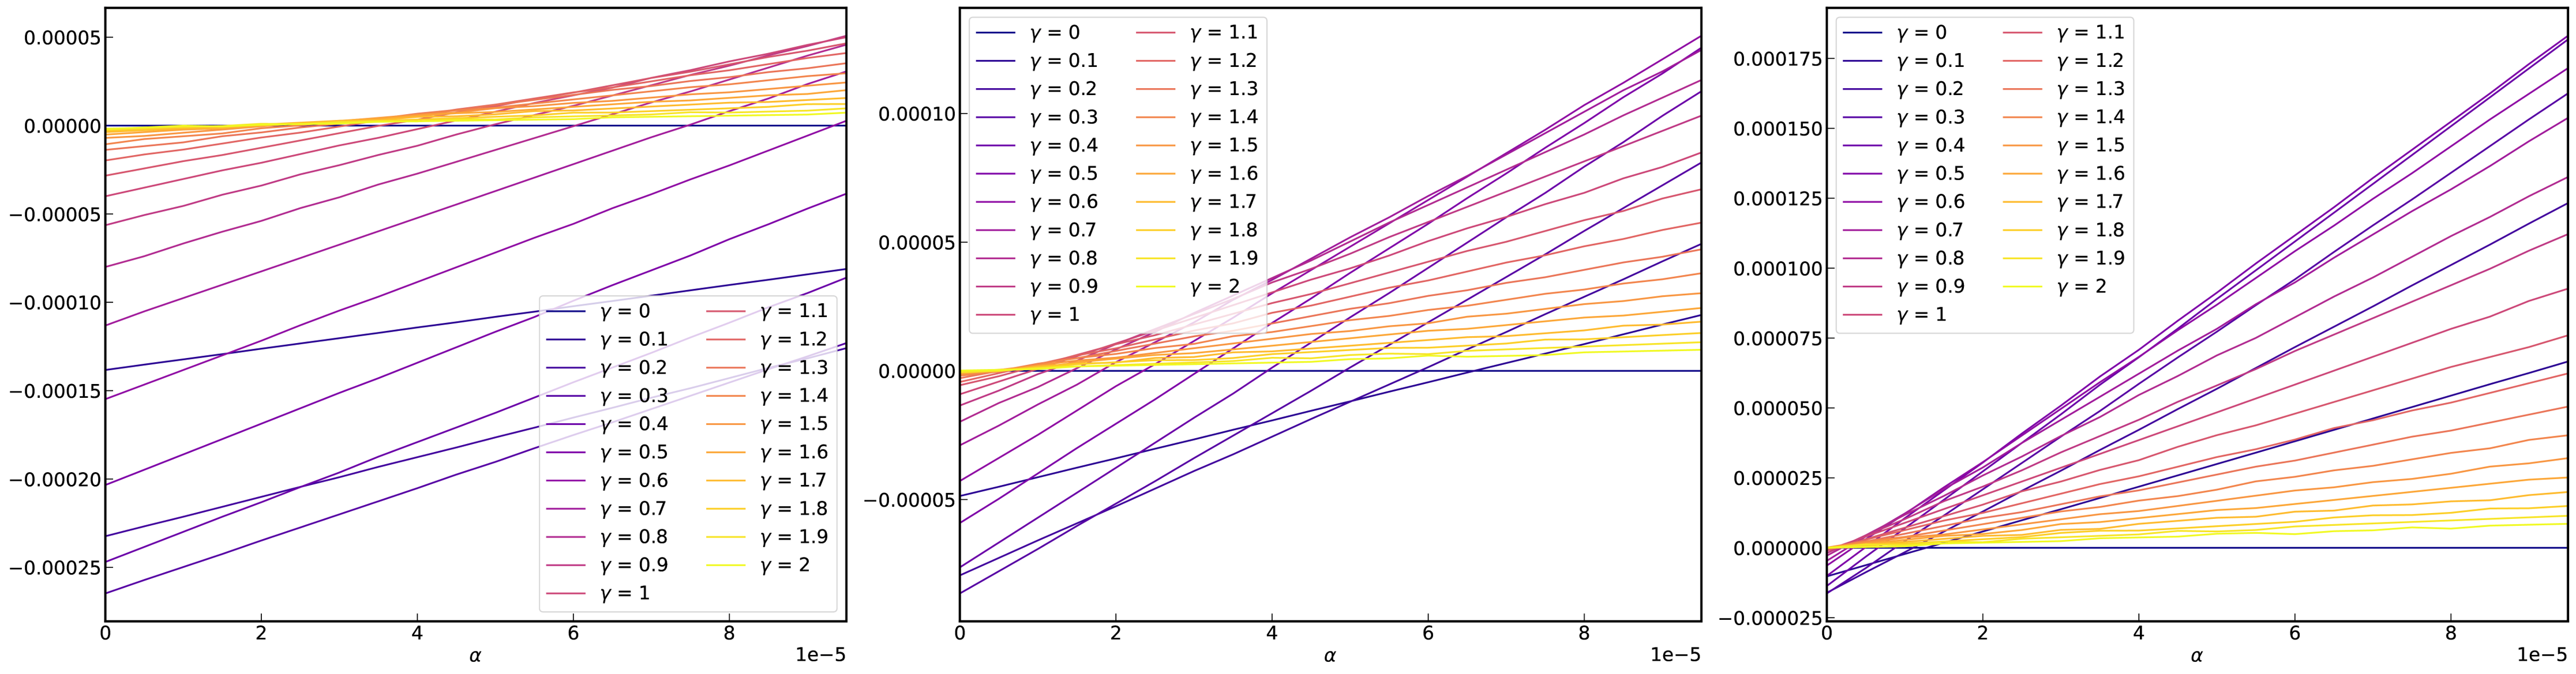
\includegraphics[width=17cm]{TexFigure/litlalp_1.png}}
  \caption{Crossover tendency calculated on NCA for fixed $\gamma$ and $T$ with varying $\alpha$ value. The temperature conditions are T = [0.14, 0.12], T = [0.12, 0.1], and T = [0.1, 0.08] 
  from left to right. As the temperature decreases, the crossover behavior of $\frac{\partial \nu}{\partial T}$ 
  at large $\gamma$ values also decreases. This implies that at low temperatures, the change of state could not occur 
  as the nonlinearity of the junction increases.}
\end{figure}
\begin{figure}[H]
  \centerline{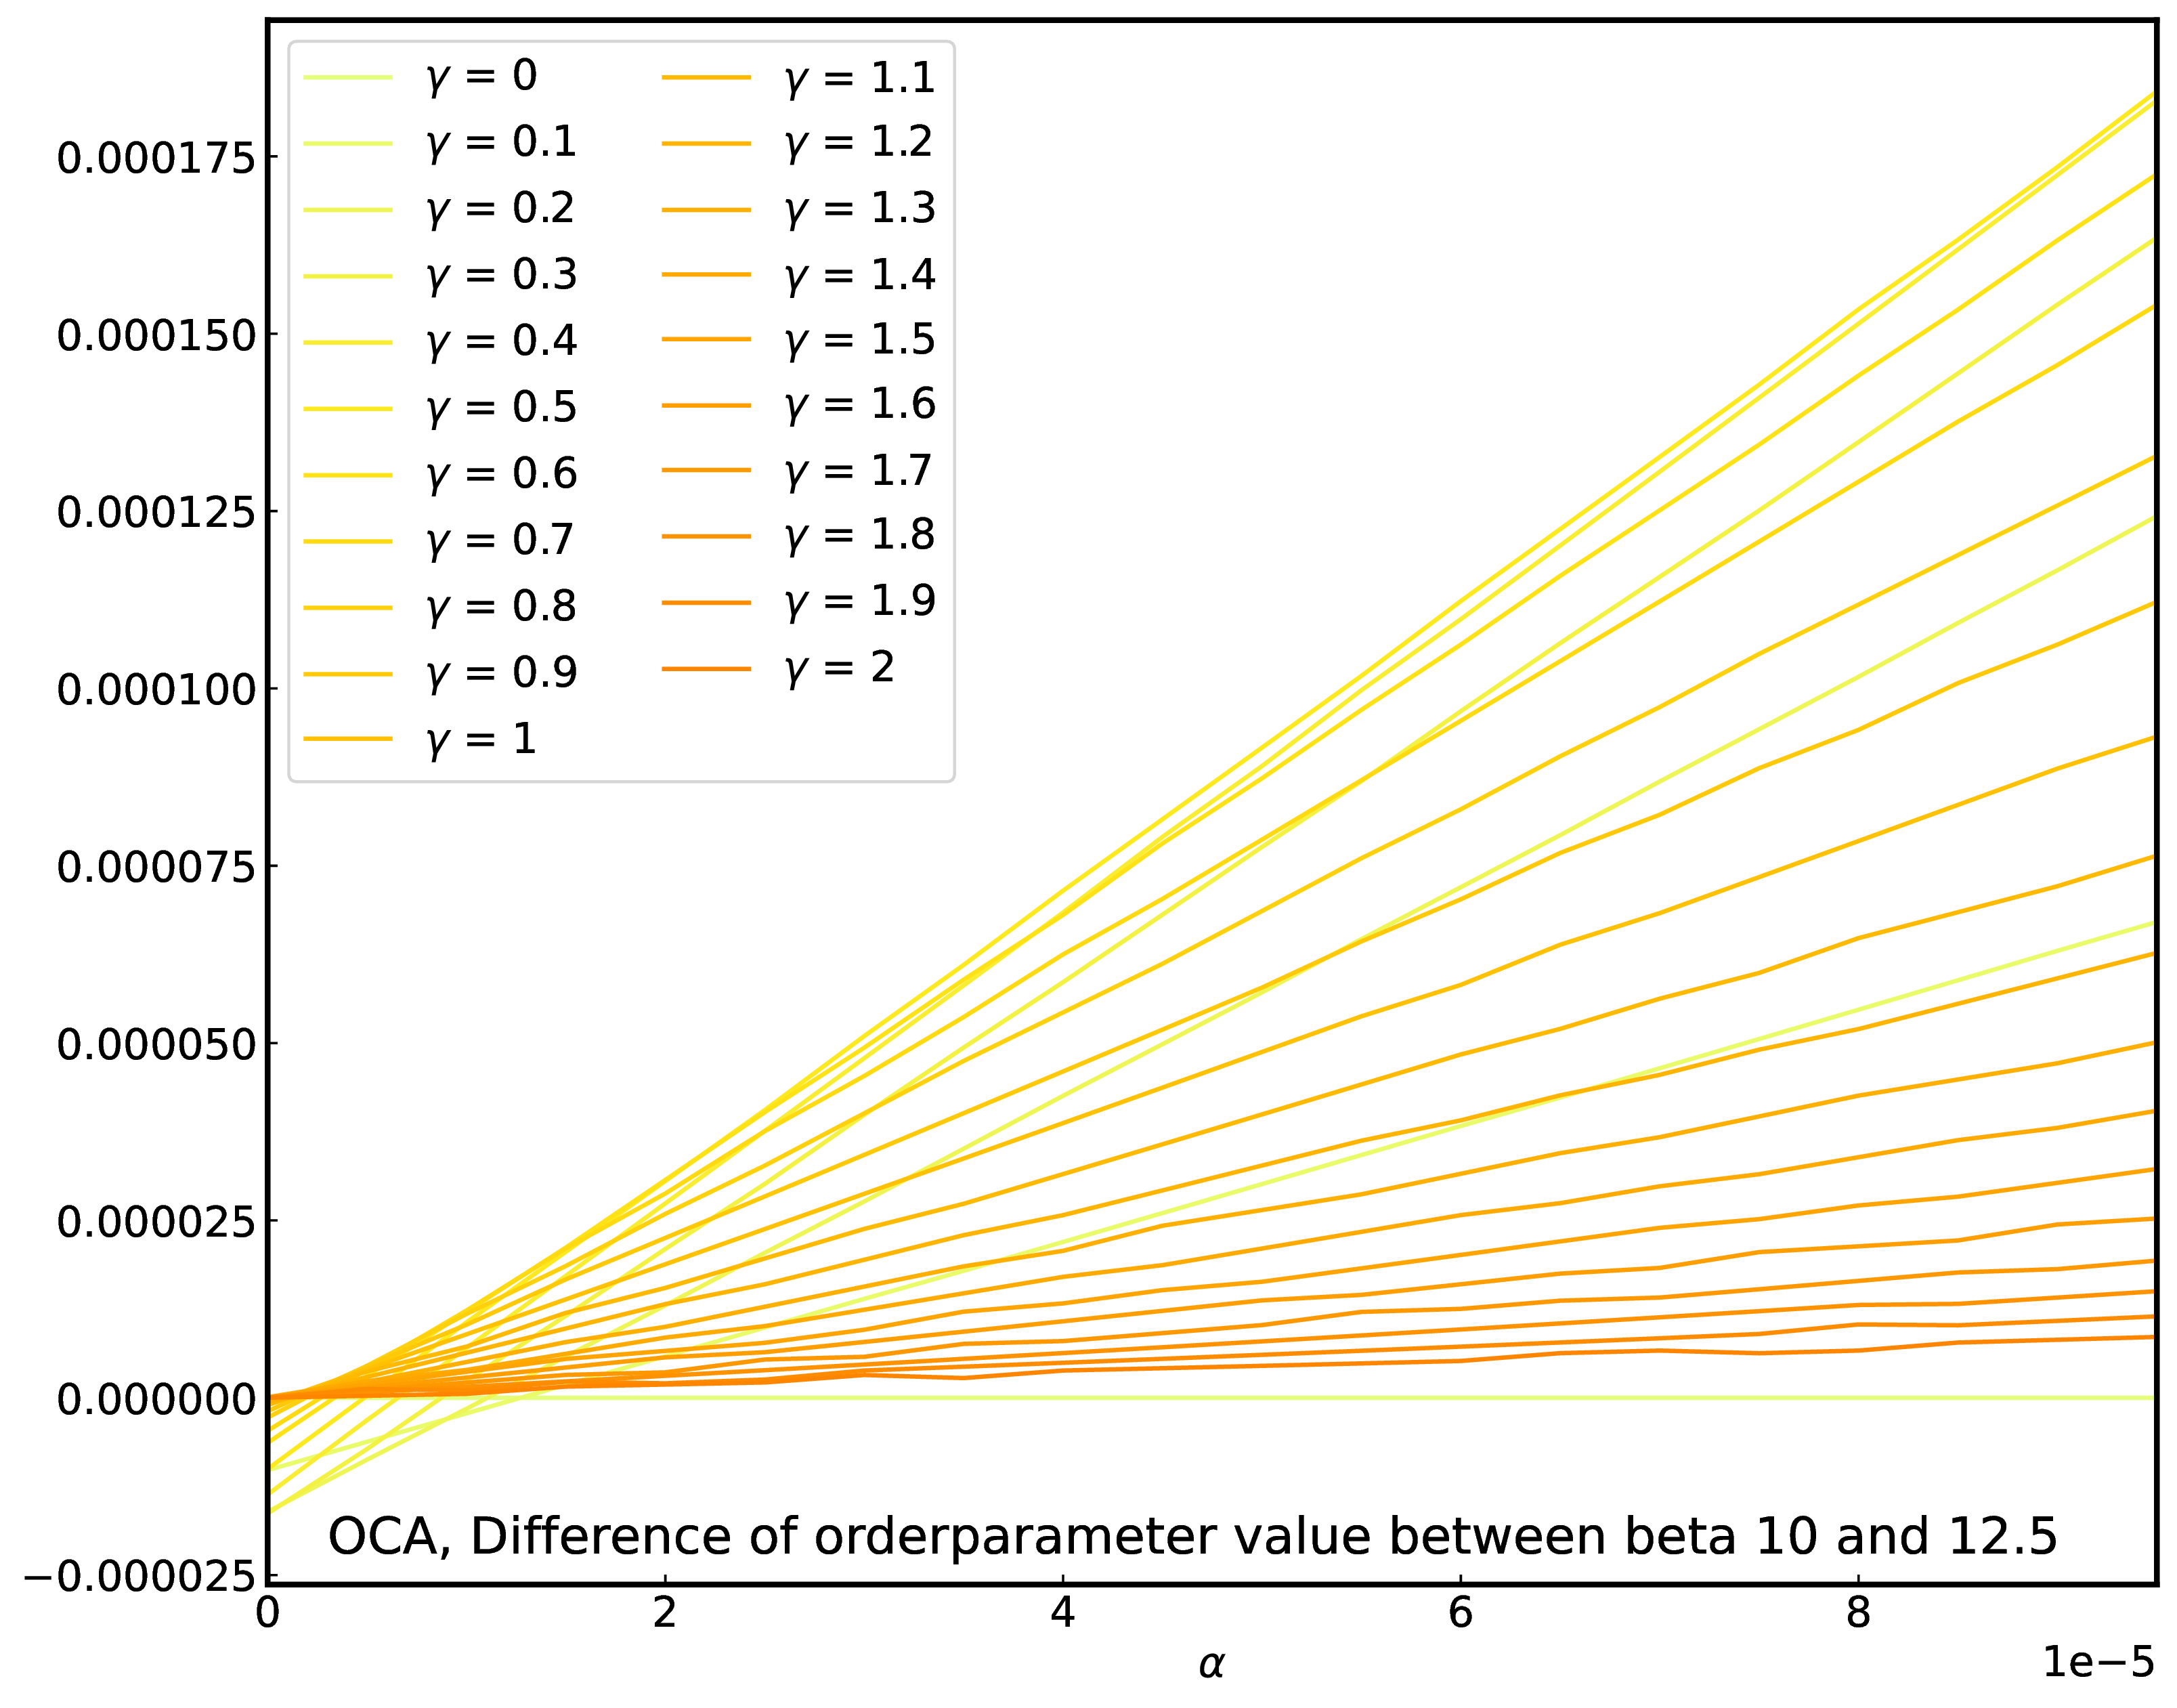
\includegraphics[width=7cm]{TexFigure/Diff_Os3_b_10_12.5_n.png}}
  \caption{Crossover tendency calculated on OCA. The consecutive temperature condition is T = [0.1,0.08].}
\end{figure}
\begin{figure}[H]
  \centerline{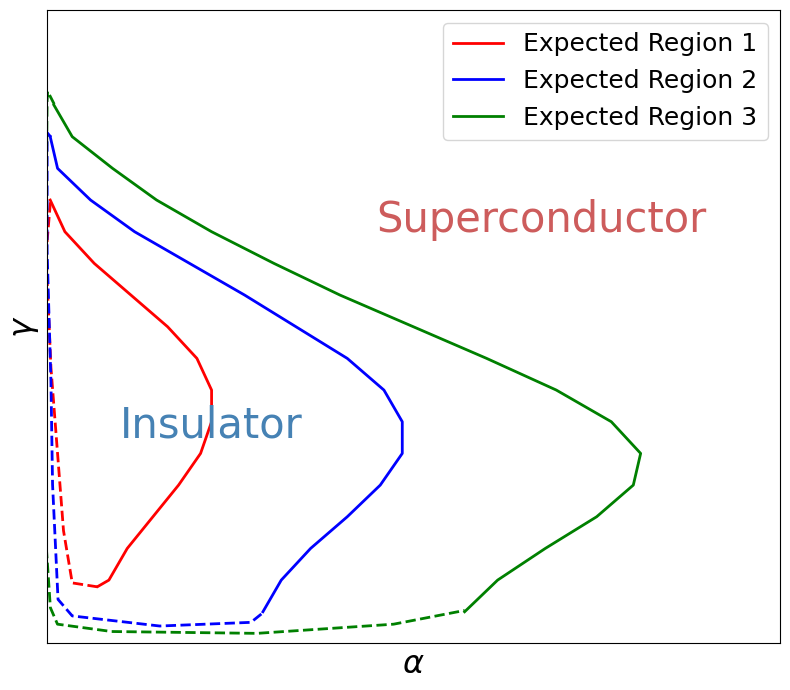
\includegraphics[width=7cm]{TexFigure/Expecregi.png}}
  \caption{Expected phase transition diagram. Expected crossover behavior is represented as a dotted line. 
  We can deduce as the temperature increases, the insulator behavior becomes wider. 
  The Red line is the highest temperature crossover line and green is the lowest temperature.}
\end{figure}
\vfill


\pagebreak
\newpage

\subsection{$\chi_{sp}$}
We utilize the method of calculating approximation frequency, which has formula:
\begin{flalign}
  \beta \chi_{sp}(\tau = \frac{\beta}{2})
\end{flalign}
Calculating the phase transition using the relationship the correlation function, 
we observed the following results: Varying the $\gamma$ value at a fixed $\alpha$ value, 
phase tended to decrease as the interaction with the external environment increased. 
In particular, at low temperatures, the phase increased up to a certain value
while the rate of change decreased with respect to the $\alpha $ value.
When we fixed the $\gamma$ value and varied the $\alpha$ value, the phase always increased at high temperatures. 
However, at low temperatures, we observed that the phase decreased as the $\alpha$ value increased.
\begin{figure}[H]
  \centerline{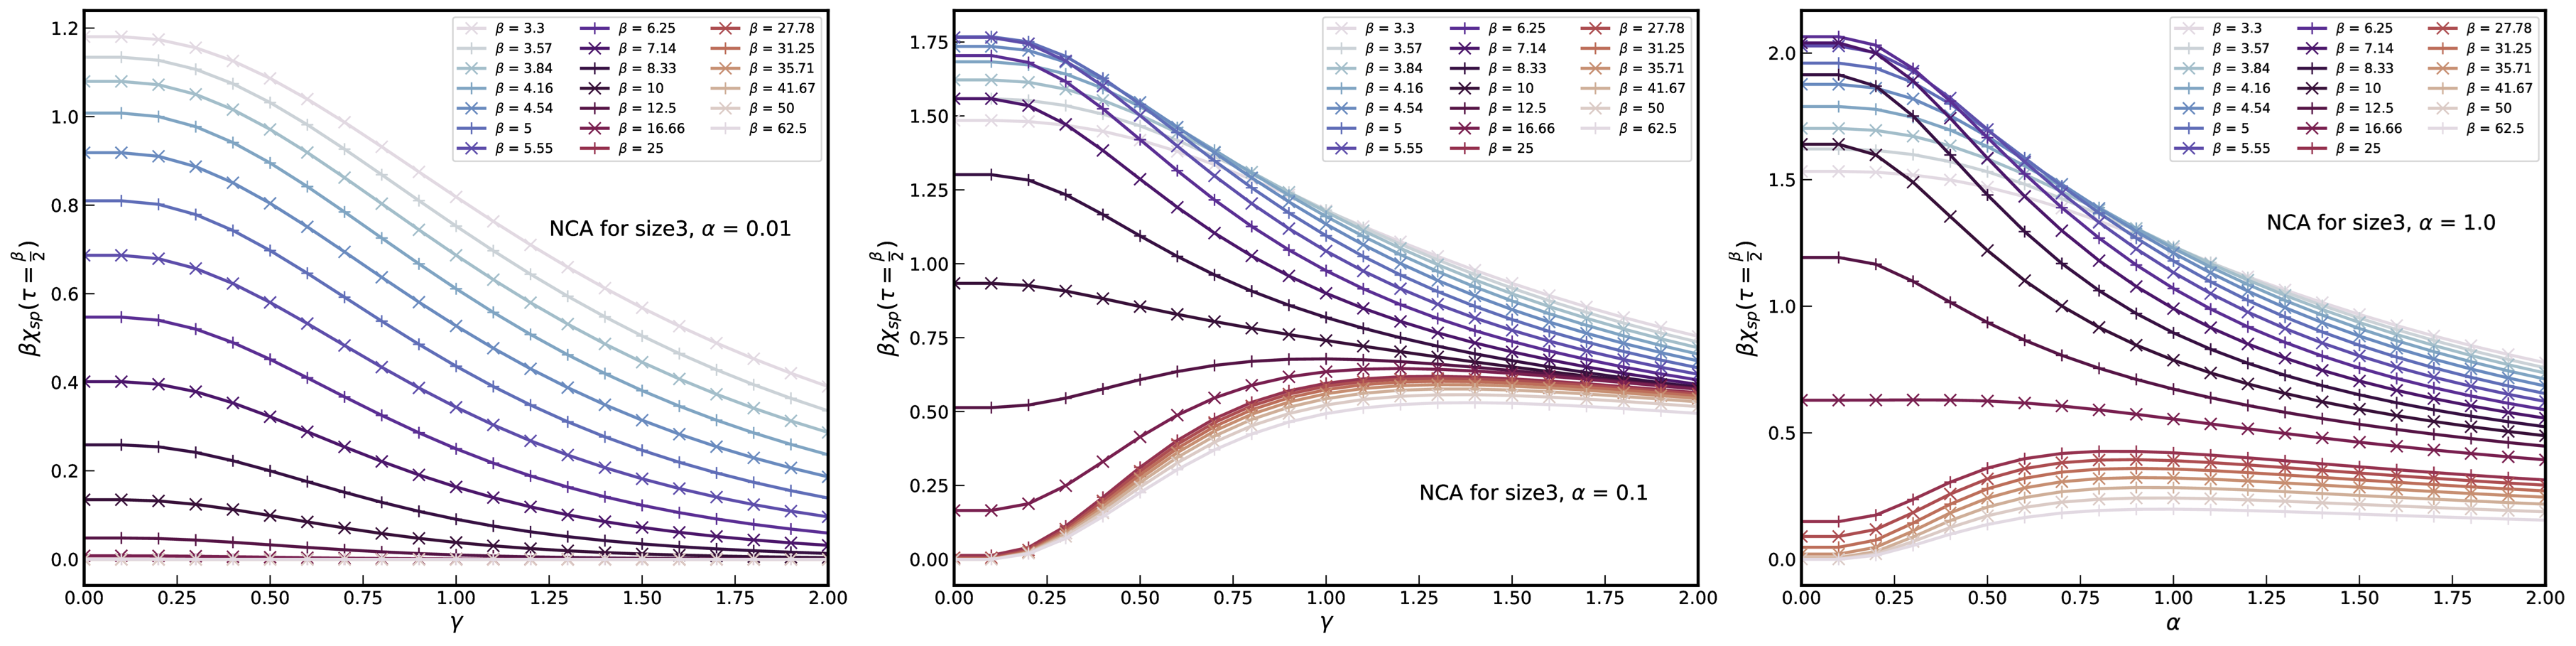
\includegraphics[width=16cm]{TexFigure/chi_gam_swp.png}}
  \centerline{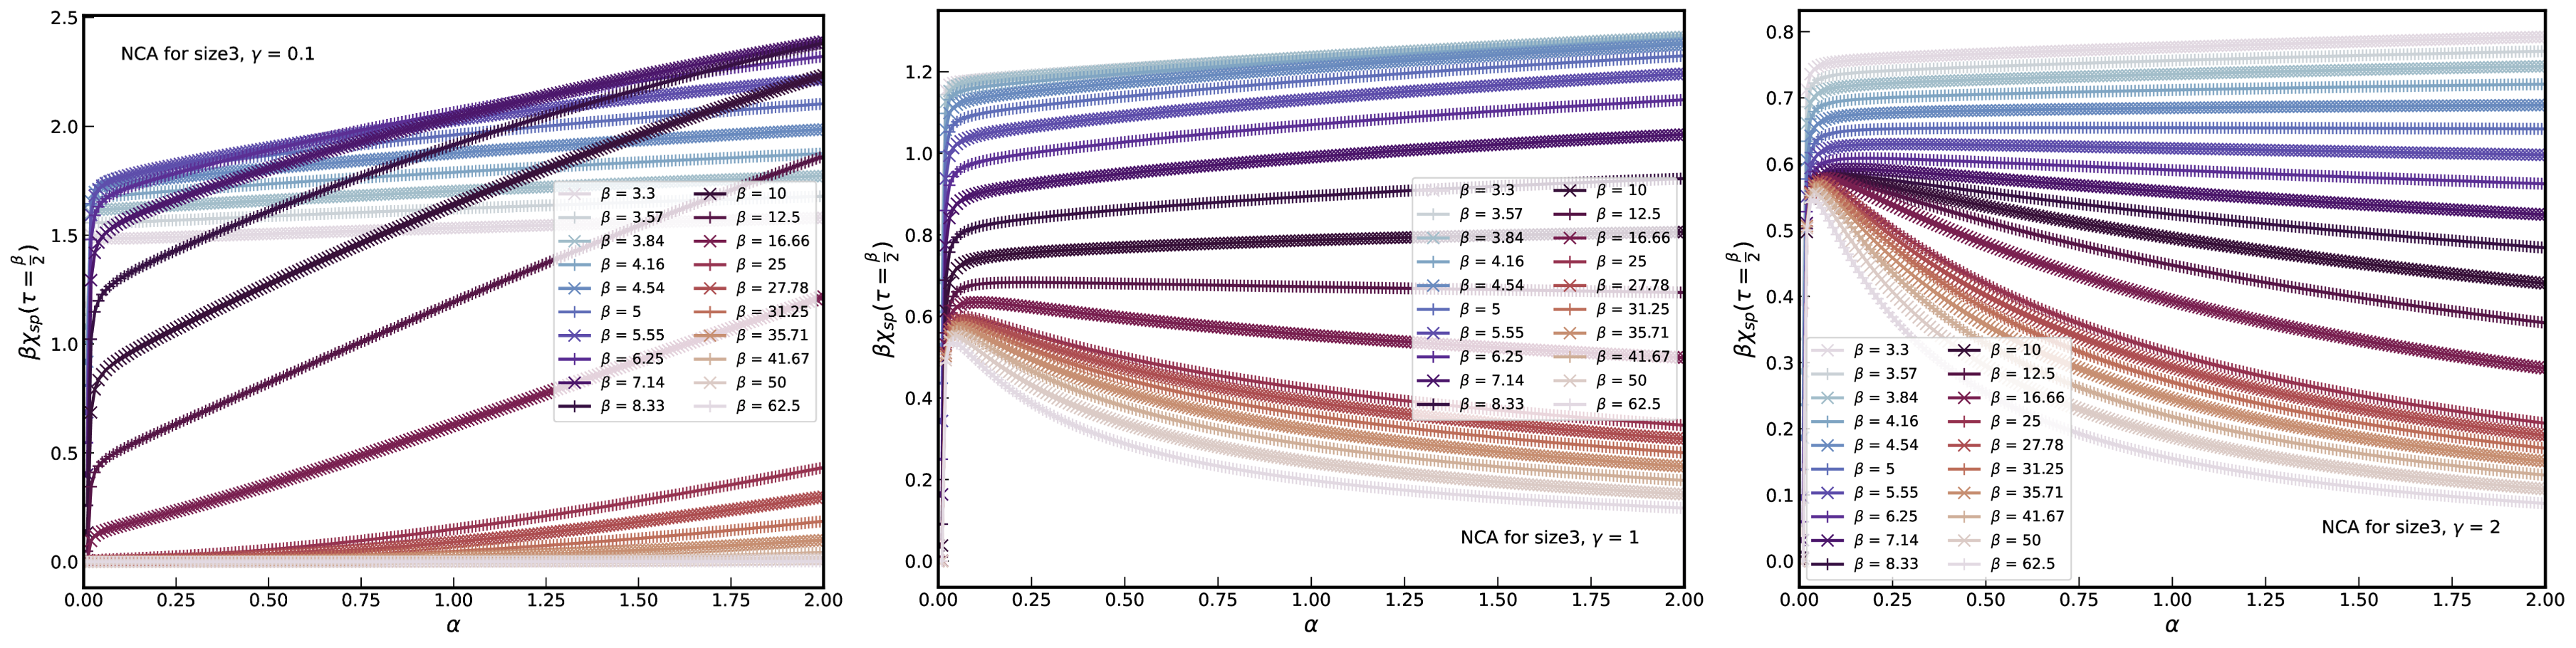
\includegraphics[width=16cm]{TexFigure/chi_alp_swp.png}}
  \caption{The crossing picture in $\chi_{sp}$ with $\gamma$ swapping and $\alpha$ swapping}
\end{figure}
\pagebreak
To observe how the phase changes for all $\gamma$ and $\alpha$ value conditions at a fixed temperature, 
we visualized the results using a 2D color map. At high temperatures, 
we observed that the phase increased as the $\gamma$ and $\alpha$ values increased. 
At low temperatures, the phase generally decreased as the influence of the external environment increased. 
Yet the junction energy increased, phase tended to increase in stronger influence from the external environment.
\begin{figure}[H]
  \centerline{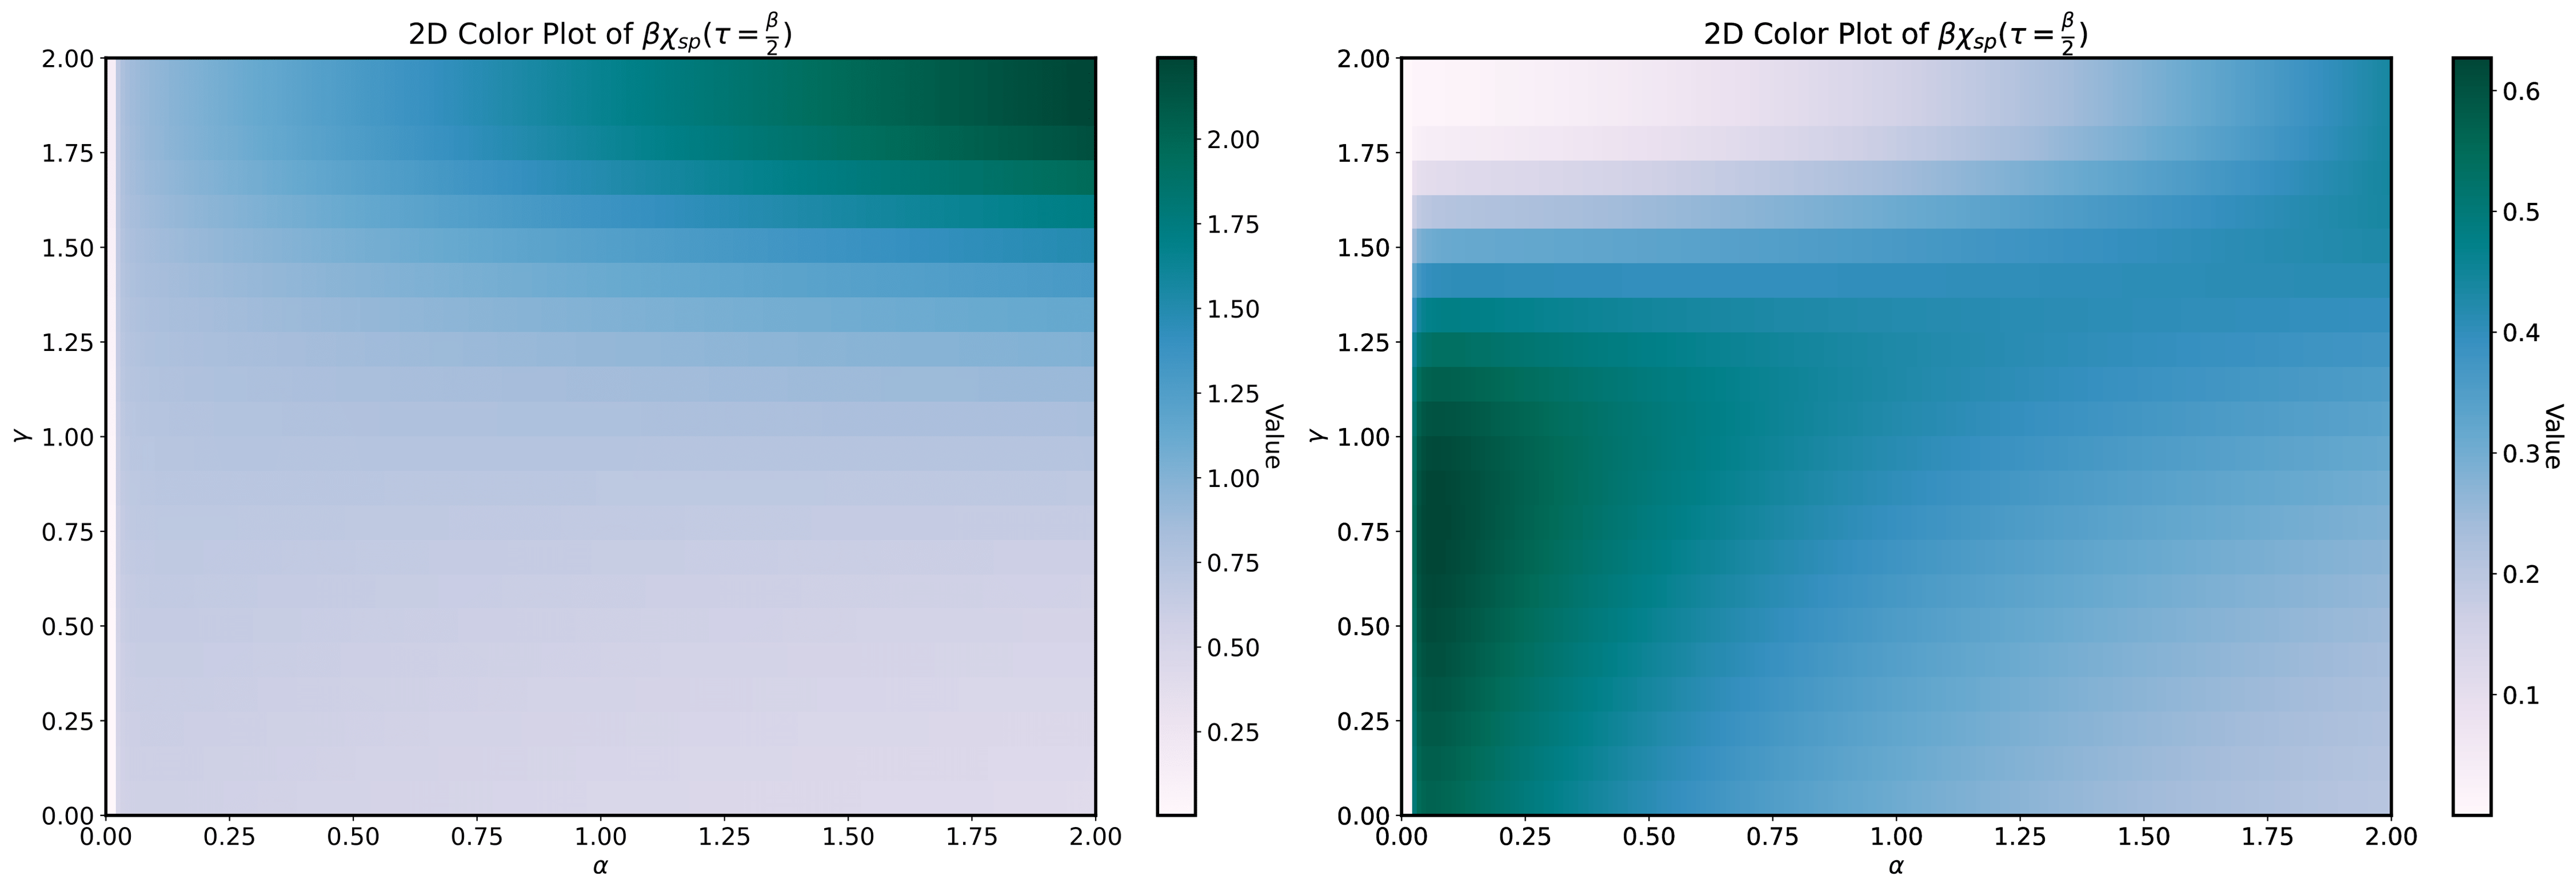
\includegraphics[width=16cm]{TexFigure/chi_color.png}}
  \caption{Colored plot for real frequency approximation. The simulation was performed in NCA. Left figure is in the case of $\beta=10$, Right is for $\beta=25$.
  The Josephson junction goes high conductivy as color goes deeper.}
\end{figure}
\pagebreak
\subsubsection*{$\chi_{sp}$ result from exceeded simulation range}
In the metal-insulator transition calculation using approximation method using correlation function, 
while plotting the temperature-dependent behavior of phase calculated with the approximation formula varying the influencing variables, 
the point where the lines crossing corresponding to two consecutive temperatures intersect can be predicted as the phase transition point.
Within the previous set simulation range, 
the temperature-dependent phase approximation behavior was not clearly observed. 
Therefore, as a first attempt, we tried calculations with a wider range of $\alpha$ values while maintaining the range of $\gamma$ values. 
However, it should be noted that the size of the $\tau$ grid was reduced for faster calculation verification. 
The range conditions used are shown in the table below.
\begin{table}[htbp]
  \centering
  \renewcommand{\arraystretch}{1.2}  % 행 간격 조정
  \begin{tabular}{@{}cccc@{}}
  \toprule
  \textbf{Variables} & \textbf{Min} & \textbf{Max}  & \textbf{Interval}\\ 
  \midrule
  $\gamma$ & 0 & 2 & 0.01 \\
  $\alpha$ & 0 & 20 & 1 \\
  $\beta$ & 3.3 & 25 &  \\
  Temperature & 0.3 & 0.04 & 0.02 \\
  \bottomrule
  \end{tabular}
  \caption{Exceeded parameter condition used for $\chi_{sp}$ calculation.}
  \end{table}
\begin{table}[htbp]
  \centering
  \renewcommand{\arraystretch}{1.2}  % 행 간격 조정
  \begin{tabular}{@{}ccc@{}}
  \toprule
  \textbf{Number} & \textbf{Interval} & \textbf{Gridsize}\\ 
  \midrule
  $\tau$ grid & [0,$\beta$] & 700 \\
  k grid & [0,K = 30000] & 30000 \\
  \bottomrule
  \end{tabular}
  \caption{Exceeded grid condition used for $\chi_{sp}$ calculation}
  \end{table}
\\
When the calculation was performed by increasing the $\gamma$ value for a fixed $\alpha$ value, crossing points occurred according to temperature, 
and it was confirmed that the points obtained within the temperature interval converged to a specific line as the $\alpha$ value increased. 
Purple lines represent the results of OCA, and green lines represent the results of NCA. 
Based on the result, we draw the expected locations of the critical points from the results calculated by the approximation method. 
The change of $\gamma$ as a function of $\alpha$ was re-plotted using the phase intersection points above. 
The color of the each line corresponds to different $\beta$ value.
Throughout the result, we confirmed that the reason why the prediction of the phase transition point through phase approximation was not possible 
in the previous calculation range was that no intersection value appeared at $\alpha$ values less than 2 at low temperatures. 
Also, we confirmed that the phase transition interval using approximation decreased as the temperature decreased.
\pagebreak
\begin{figure}[H]
  \centerline{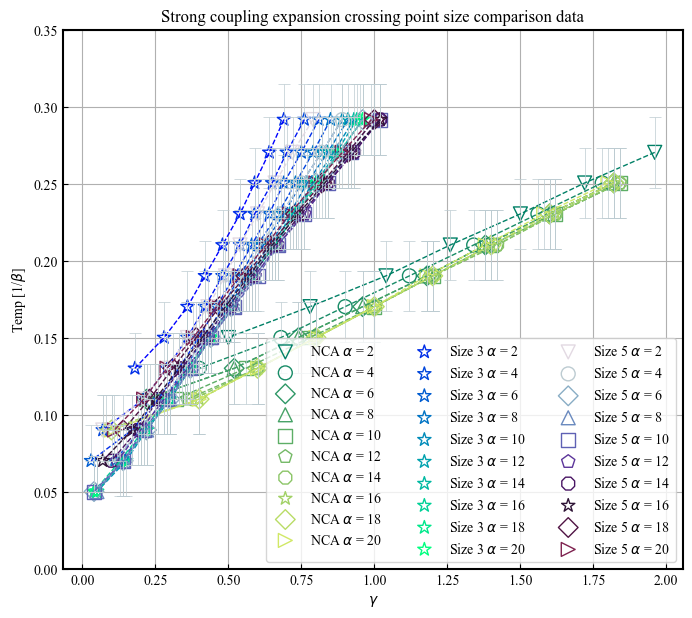
\includegraphics[width=12cm]{TexFigure/output.png}}
  \caption{Crossing points in the exceeded range. Each color represents the difference in the approximation method, 
  with green representing NCA with a matrix size of 3,  and purple representing OCA for matrix sizes 3 and 5 respectively. 
  It can be observed that the position of the line changes significantly for a matrix size of 3, i.e., a two-level energy system, 
  in the region with large $\alpha$ values.}
\end{figure}
\begin{figure}[htbp]
  \centerline{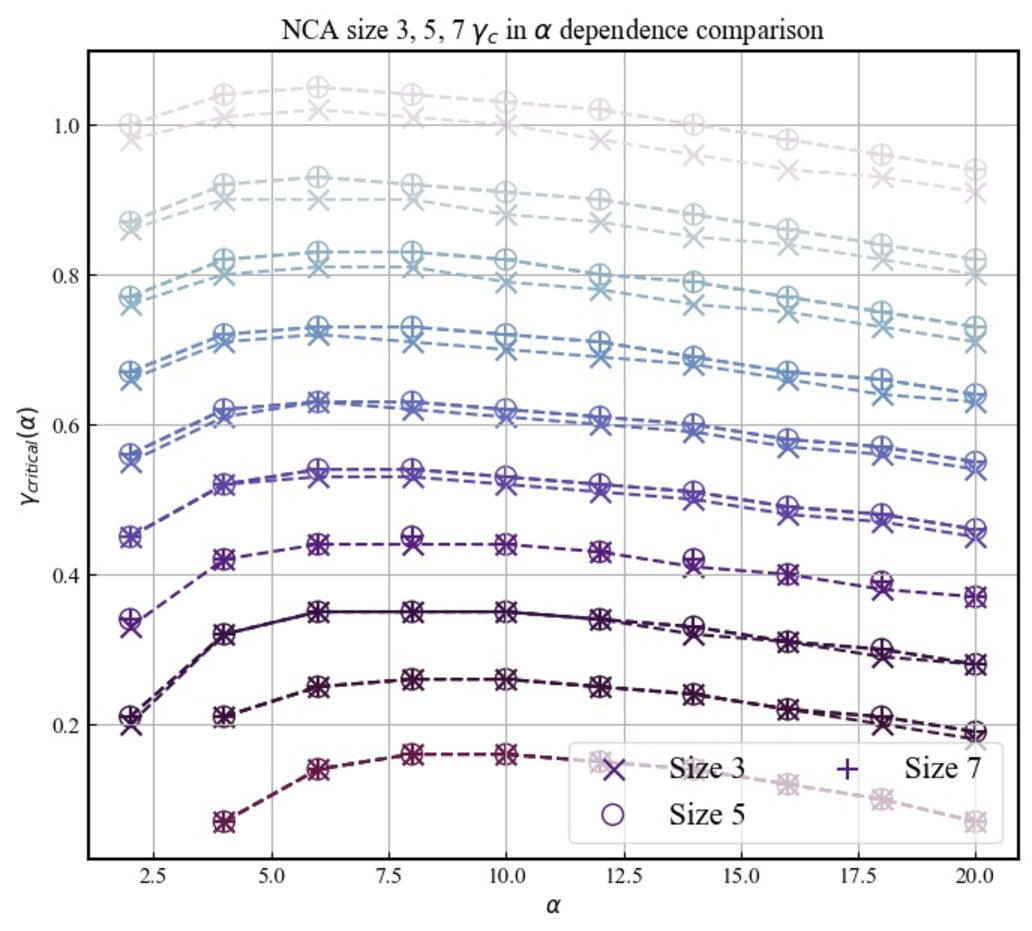
\includegraphics[width=12cm]{TexFigure/NCA_crit-7.pdf}}
  \centerline{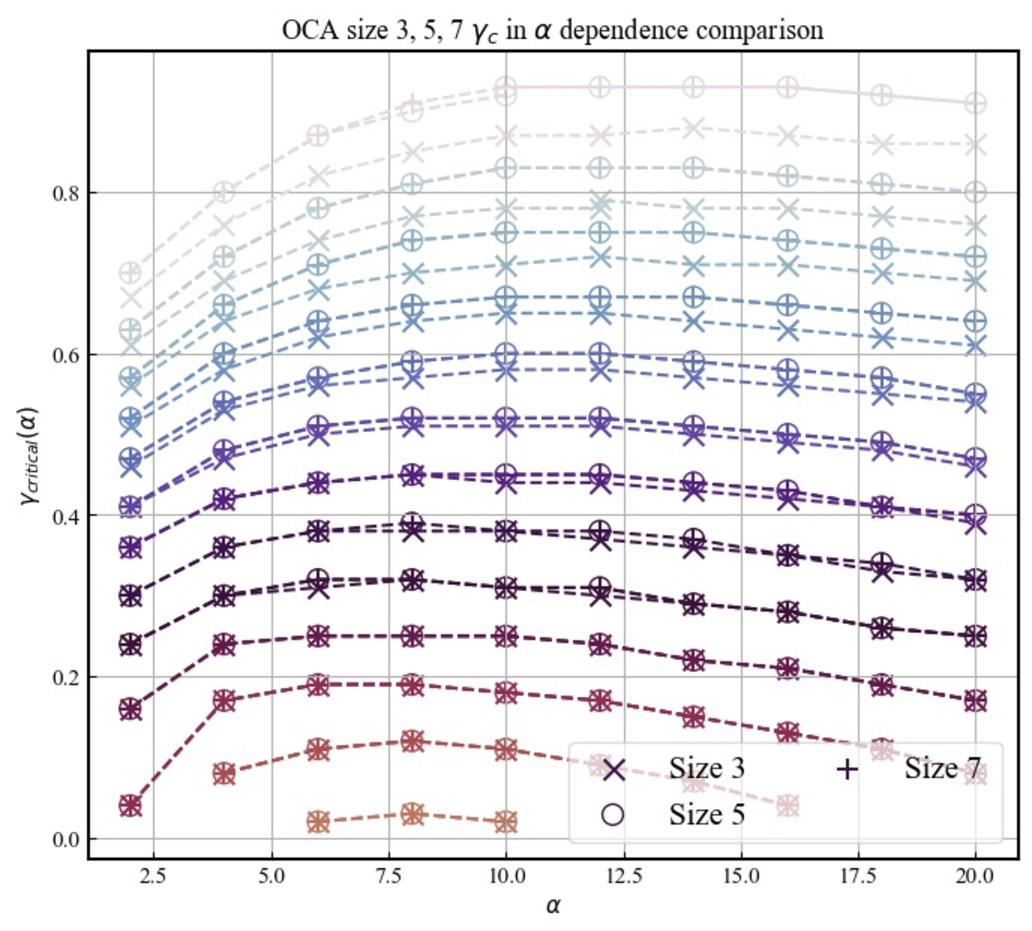
\includegraphics[width=12cm]{TexFigure/OCA_crit-7.pdf}}
  \caption{Estimated line of the criticality of the system in gamma as the function of alpha. 
  Each colored line corresponds to each temperature when the temperature range from 0.3 to 0.04 is divided into 0.02 intervals 
  from top to bottom. In the case of NCA, no critical point was observed at temperatures below 0.08.}
\end{figure}
\pagebreak
\newpage
\end{spacing}
\end{document}